\documentclass[oneside,a4paper,12pt]{book}
\usepackage{subcaption}
\usepackage[lmargin=2.8cm, rmargin=2.8cm, tmargin=3.3cm, bmargin=3.3cm]{geometry}
\linespread{1.1}
\setlength{\parskip}{1ex plus 0.5ex minus 0.2ex}


\usepackage[utf8]{inputenc}
\usepackage[spanish]{babel} % espanol
\usepackage{multirow} % Para las tablas

\usepackage{graphicx}%para imagenes
\graphicspath{ {img/} }
\usepackage{url}

\usepackage{varwidth} % cajas

\title{WebRTC Drone}
\author{Iván Rodríguez-Bobada Martín}

\usepackage{enumerate} % enumerados
\usepackage{listings}
\usepackage{color}
\definecolor{lightgray}{rgb}{.9,.9,.9}
\definecolor{darkgray}{rgb}{.4,.4,.4}
\definecolor{purple}{rgb}{0.65, 0.12, 0.82}


\lstdefinelanguage{JavaScript}{
  keywords={typeof, new, true, false, catch, function, return, null, catch, switch, var, if, in, while, do, else, case, break},
  keywordstyle=\color{blue}\bfseries,
  ndkeywords={class, export, boolean, throw, implements, import, this},
  ndkeywordstyle=\color{darkgray}\bfseries,
  identifierstyle=\color{black},
  sensitive=false,
  comment=[l]{//},
  morecomment=[s]{/*}{*/},
  commentstyle=\color{purple}\ttfamily,
  stringstyle=\color{red}\ttfamily,
  morestring=[b]',
  morestring=[b]"
}

\renewcommand{\lstlistingname}{Listado} % Cambiar pie de pagina de ingles a español

\lstset{
   language=JavaScript,
   backgroundcolor=\color{white},
   extendedchars=true,
   basicstyle=\footnotesize\ttfamily,
   showstringspaces=false,
   showspaces=false,
   frame=single,
   numbers=left,
   numberstyle=\footnotesize,
   numbersep=9pt,
   tabsize=2,
   breaklines=true,
   showtabs=false,
   captionpos=b
}






\begin{document}

\thispagestyle{empty}

\vspace{2cm}

\begin{figure}[htb]
\centerline{\resizebox{.60\textwidth}{!}{\includegraphics{img/logo-urjc}}}
\end{figure}

\vspace{8mm}
\begin{center}
{\Large {\bf Grado en Ingeniería en Sistemas Audiovisuales y Multimedia}}
\vspace{8mm}

{\large Escuela Técnica Superior de Ingeniería de Telecomunicación}
\vspace{8mm}

{\large Curso académico 2015-2016}

\vspace{1.0cm}

{\large {\bf Trabajo Fin de Grado}} 

\vspace{2cm}
{\Huge {Manejo de un drone con WebRTC y JdeRobot}}

\end{center}

\vspace{4cm}
\makebox[11cm][r]{
\begin{tabular}{ll}
{\bf Autor}: & Iván Rodríguez-Bobada Martín \\
{\bf Tutor}:& José María Cañas Plaza \\
\end{tabular} 
}

\vspace{0.5cm}
\begin{center}
\large{Madrid 2015}
\end{center}



\clearpage
\thispagestyle{empty}

\vspace{5cm}
\makebox[15cm][r]{
\begin{tabular}{ll}
&\emph{A mis padres y hermanos,}\\
&\emph{que siempre han estado a mi lado,}\\
&\emph{y siempre lo estarán.}\\
&\\
&\emph{Y a mis amigos, por ser }\\
&\emph{verdaderamente mis amigos.}\\
&\\
&\emph{Gracias.}
\\
\end{tabular}
}

\let\OLDthebibliography=\thebibliography
\def\thebibliography#1{\OLDthebibliography{#1}%
  \addcontentsline{toc}{chapter}{\bibname}}

\tableofcontents
\listoffigures


\chapter{Introducción}

El proyecto que explica esta memoria se encuadra dentro del manejo, control, recogida y procesado de datos de sensores y actuadores de un drone a distancia. El drone es un vehículo aéreo no tripulado al que podemos definir dentro de la robótica aérea. En las siguientes páginas se dará unas pinceladas sobre la robótica, su historia y uso actual. También hablaremos sobre los sistemas actuales de control y manejo del drone, y para finalizar daremos una visión global sobre las tecnologías existentes dentro de las Comunicaciones en Tiempo Real (RTC, Real Time Communications).\\

\section{Robótica}

\section{Sistemas de control de drones}

Los drones pertenecen a la rama de robótica aérea, y a su vez dentro de los vehículos aéreos es un vehículo aéreo no trupilado (UAV, Unmanned  Aerial Vehicle).Es un vehículo no tripulado, pero no autónomo, por lo que necesitan ser teleoperados desde tierra. Los sistemas actuales para ello se pueden dividir en dos grupos, los controlados mediante radiofrecuencia y los que usan sistemas propietarios.\\

\subsection{Radiocontrol}

Es la técnica que permite el gobierno de un objeto a distancia de manera inalámbrica mediante una emisora de control remoto. Por otra parte, a bordo del vehículo, en nuestro caso un drone, debe ir una receptora de radio control. \\
***IMAGEN***
La comunicación entre receptor y transmisor se efectúa mediante radiofrecuencia, existiendo diferentes sistemas de emisión, como AM, FM o 2.4Ghz con diferentes tipo de codificación, PCM, PPM…\\

Estos sistemas tienen varias limitaciones. Una es el número de canales máximo del sistema, ya que se usa un canal para cada elemento de control disponible: elevación, giro, rotación… La segunda y posiblemente más crítica son las interferencias. Si se producen interferencias ya sea por ruido o por varios emisores trabajando en las cercanías se puede perder el control de la aeronave y destruir la misma o incluso dañar a personas.\\
 
\subsection{Sistemas alternativos}

En la actualidad a parte del radiocontrol tenemos el control a través de WiFi. Este sistema consiste en la creación de una red WiFi por parte del drone a la cual se conecta el dispositivo con el que se maneja. Este dispositivo puede ser un mando diseñado y comercializado por la propia marca o un dispositivo móvil, el cuál usa una aplicación que es la que gestiona la conexión y transferencia de datos.\\

Empresas como DJI usa sistemas mixtos que consisten en teleoperar el drone vía radiocontrol, pero la gestión de la cámara, con visualización incluida.\\
 
La empresa francesa Parrot, la cual tiene una flota de diversos modelos de drones, utiliza un sistema de red WiFi, a la cuál conectas un dispositivo móvil ya sea Android o iOS, y mediante una aplicación desarrollada por ellos se puede controlar el drone, así como tener otras funcionalidades como la grabación de video, captura de imágenes y gestión de parámetros de vuelo como altura o velocidad máxima. En capítulos posteriores profundizaremos en este sistema implementado, ya que es el que usaremos para desarrollar el nuestro.\\
 
\section{Tecnologías de comunicación a distancia en tiempo real}

\section{Motivación}

\chapter{Objetivos}

Una vez situado el Trabajo Fin de Grado en su contexto vamos a presentar los objetivos que nos marcamos para la realización del mismo. Los objetivos a abordar son tres, los cuáles expongo a continuación.

\section{Objetivos}
\subsection{Conexión local}

Como primer objetivo tenemos que desarrollar una conexión directa con el drone. Esta conexión tiene que ser bidireccional, ya que tenemos que acceder a los sensores y actuadores del drone, así como a su cámara, pero también es necesario mandarle ordenes de movimiento.\\

Como requisito fundamental para esta conexión es que tiene que ser en tiempo real y que sea lo suficientemente fluida y ligera como para que no introduzca ningún tipo de retardo.\\


\subsection{Conexión remota}

El segundo punto con el que nos enfrentamos es utilizar una tecnología web moderna y actual con la que poder teleoperar el drone. Esta tecnología tiene que ser lo suficientemente versátil como para poder implementarla en nuestro proyecto. Por otro lado, al igual que la conexión local, tiene que ser bidireccional, poder transportar audio y vídeo e introducir el mínimo retraso en la comunicación posible para tener una experiencia positiva y controlada del vuelo del drone.\\

Esta conexión deberá realizarse entre el ordenador local y un segundo ordenador, que será desde el que el usuario podrá teleoperar el vehículo.\\

Durante toda la memoria nos referiremos como ordenador local, par local o navegador local al dispositivo que usaremos para conectarnos al cuadricoptero y el cuál deberá ir a bordo del drone, y ordenador remoto, par remoto o navegador remoto al ordenador desde el cuál teleoperaremos el vehículo.\\

Como sub-objetivos para esta conexión tenemos los siguientes:

\begin{itemize}

\item \emph{Visualización de cámara a bordo:} La conexión tiene que ser capaz de transportar el flujo audiovisual de la cámara del drone desde el navegador local hasta el navegador remoto.

\item \emph{Sensores de navegación.} Los datos obtenidos de los sensores de navegación del cuadricoptero deberán ser enviados al ordenador remoto donde se visualizaran.

\item \emph{Localización espacial del drone.}La brújula y GPS del cuadricóptero deberán ser recogidas por el ordenador local, y deberán enviarse al ordenador remoto para poder visualizar en este un mapa para tener localizada la posición del vehículo.

\item \emph{Ordenes}. Desde el ordenador remoto deberán enviarse hacia el ordenador local las ordenes dadas para el aterrizaje, despegue, y comandos de movimiento.


\end{itemize}

De manera general el par local deberá establecer la conexión con el drone, acceder a sus sensores y a su cámara. Deberá también establecer una conexión con el ordenador remoto y enviarle todos estos datos obtenidos del drone. Del par remoto recibirá las ordenes y comandos de movimiento, que deberá enviárselos al drone.\\

El par remoto deberá establecer la conexión con el par local. De este recibirá todos los datos del drone y deberá representarlos de una manera que el usuario final pueda conocer la situación de vuelo del drone en cada momento. Deberá tener una interfaz amigable que le permita recoger las órdenes de movimiento dadas por el usuario, y enviárselas al par local.\\

En la figura \ref{fig:esquemageneral} tenemos un esquema de la estructura general del proyecto.\\

\begin{figure}[htb]
\centering
\includegraphics[width=0.9\textwidth]{conexiones}
\caption{Esquema general del proyecto}
\label{fig:esquemageneral}
\end{figure}

\subsection{Interfaz amigable y actual}

Uno de los requisitos es desarrollar una interfaz clara, que nos muestre de una manera lo mas realista, clara y concisa posible los datos recogidos de los sensores del drone y la cámara para permitirnos conocer el estado de vuelo del drone en cada momento: altitud, inclinación, velocidad...\\


Para que la satisfacción de vuelo sea satisfactoria la interfaz tiene que tener unos controles de movimiento que sean sencillos, simples e intuitivos.\\

Esta interfaz deberá realizarse con tecnología web actual y moderna, y deberá permitirnos el manejo del cuadricóptero de la forma mas realista y similar posible a los sistemas de control de drones que hemos hablado en el capítulo \ref{cap:controldrones}.\\

\section{Metodología y plan de trabajo}

La realización de un proyecto requiere de una metodología que establezca las pautas a seguir y la planificación de las tareas que se deben llevar a cabo para cumplir los objetivos del mismo. Hemos escogido el modelo de \emph{desarrollo en espiral}, ya que es un modelo ampliamente usado en la ingeniería de \emph{software}. Este modelo define una serie de ciclos que se repiten en un bucle hasta el final del proyecto, dividiéndolo en varias subtareas más sencillas y estableciendo puntos de control al final de cada iteración en los que se evalúa el trabajo realizado y se enfocan las nuevas tareas para continuar.\\

Esta metodología recibe su nombre por la forma de espiral que tiene su representación gráfica o diagrama de flujo, que podemos ver en la figura \ref{fig:planificacion_espiral}. En cada iteración se llevan a cabo las siguientes actividades:

\begin{itemize}
 \item \textbf{Determinar los objetivos}, dividir en subobjetivos y fijar requisitos.
 \item \textbf{Analizar los riesgos} y factores que impidan o dificulten el trabajo y las consecuencias negativas que este
 pueda ocasionar.
 \item \textbf{Desarrollar} las tareas para lograr los objetivos según los requisitos especificados.
 \item \textbf{Planificar} las próximas fases tras evaluar el transcurso del proyecto.
\end{itemize}

\begin{figure}[htb]
\centering
\includegraphics[width=0.9\textwidth]{espiral}
\caption{Esquema general del proyecto}
\label{fig:planificacion_espiral}
\end{figure}

Durante el ciclo de vida del proyecto se han hecho reuniones periódicas con el tutor. En ellas se evaluaban los avances logrados y se marcaba la hoja de ruta a tomar para los siguientes días de desarrollo. Si los puntos marcados en sesiones anteriores no se habian finalizado se ampliaba el plazo o se intentaba buscar otra manera de avance.\\

Para facilitar el seguimiento del proyecto se ha hecho uso de un mediawiki\footnote{http://jderobot.org/Irodmar-tfg} de JdeRobot en el que se iba actualizando cada avance que se lograba, con explicaciones y vídeos e imágenes. Se ha utilizado la plataforma Github\footnote{https://github.com/RoboticsURJC-students/2015-tfg-irodmar}, que es un sistema de control de versiones para alojar el código de todo el proyecto.\\

El plan de trabajo para todo el proyecto se puede dividir en las siguientes etapas:

\begin{itemize}
\item \textbf{Familiarización con JdeRobot}: Primer contacto con esta plataforma y sus herramientas para conocer su funcionamiento.
\item \textbf{Aprendizaje de tecnologías web necesarias:} Conocer las tecnologías web que van a ser necesarias para el desarrollo del proyecto. Entre ellas se encuentra WebRTC, HTML5, CSS3, WebGL, ThreeJS, o jQuery. Primer contacto también con el \emph{middleware} ICE.
\item \textbf{Desarrollo de la conexión local:} Creacion de toda la infraestructura necesaria para la interconexión entre el navegador local y el drone.
\item \textbf{Desarrollo conexión remota}: Desarrollo de la conexión remota que interconectara los dos pares.
\item \textbf{Desarrollo interfaz}: Desarrollo de la interfaz amigable para teleoperar el drone.
\item \textbf{Experimentos}: Primero se realizan pruebas con el simulador, y cuando el código este suficientemente maduro se prueba con un drone real.
\end{itemize}







\chapter{Infraestructura Software} 

Una vez presentados los objetivos que tenemos marcados hay que echar una mirada a las tecnologías software que tenemos disponibles para utilizarlas como base y pilares del proyecto. La más importante y sobre la que está centrado el proyecto es WebRTC. Luego utilizaremos, como apoyo para cubrir las partes que WebRTC no llega, ICEJS junto con la infraestructura que tiene ya desarrollada JdeRobot.


\section{WebRTC}

WebRTC es un proyecto opensource y gratuito que nos permite tener en el navegador tecnología en tiempo real ('Real-Time Communication' ó RTC), sin plugins, a través de una simple API de JavaScript. Facilita las llamadas de voz, videollamadas, chat y compartimiento de archivos y datos. WebRTC es una tecnología Peer-to-Peer, por lo que nos permite desarrollar estas aplicaciones para que funcionen directamente desde un navegador a otro sin pasar por servidor intermedio. \\

En todo el documento nos referimos a una llamada WebRTC entre dos navegadores, pero hay que tener en cuenta que en muchas ocasiones la conexión puede ser entre un navegador y algún tipo de servidor ó MCU configurado y trabajando con la API de WebRTC para ofrecernos cualquier servicio en tiempo real.\\

La API de WebRTC nos proporciona todo el set completo de funciones para manejar y crear nuestras aplicaciones, como el control y administración de la conexión, codificación/decodificación del audio/vídeo, negociación entre navegadores, control de la conexión, firewall y NAT traversal.\\

Que WebRTC no necesita un servidor no es del todo cierto, ya que sí que necesita de lo que llamamos Servidor de Señalización. Este es el encargado de establecer el primer contacto entre ellos, facilitando el intercambio de paquetes de la negociación WebRTC.\\

WebRTC está compuesto de 3 API's:

\begin{itemize}
\item getUserMedia
\item RTCPeerConnection
\item RTCDataChannel
\end{itemize}

A continuación vamos a desgranar y explicar como funciona el intercambio de paquetes de señalización así como cada una de las API's que componen WebRTC.

\subsection{Señalización} 

Señalización es el proceso de intercambio de datos y metadatos necesarios para coordinar una llamada entre navegadores con WebRTC. Para realizar esta labor WebRTC necesita de la ayuda de un servidor externo ya que la norma deja el campo de la señalización a la capa de la aplicación.\\

Entre las labores de la señalización se encuentran la detección de los peers, el intercambio de paquetes de control de la sesión como los \textit{ICE candidates} y los \textit{SDP (Session Description Protocol)}, las prestaciones que puede darnos cada peer así como cualquier otro dato o paquete necesario para realizar este 'apretón de manos' inicial.\\

WebRTC no especifica que tipo de servidor hemos de usar para estas funciones. Esto es debido a que diferentes aplicaciones pueden preferir diferentes servidores básicos o personalizados según sus necesidades. La única restricción es el uso de la arquitectura JSEP, la cuál especifica cómo debe ser la secuencia de señalización para tener una llamada exitosa.

\subsubsection{Arquitectura \textit{JSEP (JavaScript Session Establishment Protocol)}}

El servidor debe usar la arquitectura JSEP. Esta arquitectura elimina al navegador de casi todo el flujo de señalización, el cual se maneja desde JavaScript haciendo uso de dos interfaces: transfiriendo los SDP local/remoto e interactuando con la maquina de estados ICE. Esta arquitectura nos evita, entre otras cosas, que el navegador tenga que guardar estados de sesión, de tal manera que se pueden guardar en el servidor y evitar problemas si la página se recarga, por ejemplo. \\

Como ya hemos comentado, JSEP no establece un modelo particular de señalización más allá de usar uno capaz de realizar el intercambio de los SDP y ICE según la norma RFC3264 de oferta/respuesta, de tal manera que ambas partes de la llamada sepan como actuar en cada momento. JSEP nos da los mecanismos necesarios para crear estas ofertas, así como aplicarlas a las sesión.\\

El orden en que se llaman a estas mecanismos o funciones de la API es importante, por lo que la aplicación deberá saber el orden en el que tiene que llamar a cada una, convertir las ofertas en mensajes que entienda el protocolo de señalización elegido y hacer la conversión inversa con los mensajes que se reciben para obtener ofertas que entiendan as API's.\\

El manejo de las \textit{session descriptions} es simple y sencillo. Siempre que el intercambio de una oferta/respuesta es necesario, el peer que establece la llamada ó \textit{caller} crea la oferta llamando a la función \emph{createOffer()} de la API. Esta oferta puede ser modificada por la aplicación si así fuese necesario y se establece como configuración local en ese peer con \emph{setLocalDescription()} y se envía al peer remoto a través del servidor de señalización utilizado. Al recibir esta oferta el peer \textit{called} lo utiliza como configuración del otro peer con \emph{setRemoteDescription()} y utiliza \emph{createAnswer()} para crear una respuesta apropiada, la cual establece como configuración local (\emph{setLocalDescription()}) y envía la respuesta de vuelta a través del servidor de señalización. El caller al recibir la respuesta llama también a \emph{setRemoteDescription()}, y de esta manera ambos lados tienen la información del media propia y la del peer remoto.\\


\subsubsection{Descriptores de Sesión y Máquina de Estados}

Para establecer un intercambio de media, el \textit{user agent} del navegador necesita parámetros específicos para indicar al peer remoto qué es lo que va a transmitir, de la misma manera que necesita saber el media que va a recibir para saber como decodificarlo y manejarlo. Estos datos se determinan en la descripción de sesión (SDP), los cuales se intercambian en ofertas/respuestas usando las API's JSEP como ya hemos visto anteriormente.\\

Si el SDP pertenece a la parte local o remota tiene su importancia. Una vez realizado el intercambio, cada parte mirará la lista de codecs soportados por él mismo y por la otra parte, y el cruce de los resultados determinará que codecs debe enviar y cuál espera recibir. Como podemos intuir, los parámetros exactos de la transmisión solo se pueden saber una vez la oferta y la respuesta han sido intercambiados. Sin embargo, hay ocasiones en las que el caller o el que hace la oferta puede recibir media después de enviar esta pero antes de recibir la respuesta de la otra parte. Para procesar este media de manera adecuada, el manejador de caller debe conoce los detalles de la oferta antes de que la respuesta llegue.\\

Por lo tanto, para manejar los session description de manera correcta, los user agent necesitan:

\begin{itemize}
\item Conocer si el session description pertenece a la parte local o remota.
\item Conocer si el session description es una oferta o una respuesta.
\item Permitir a la oferta ser especificada independientemente de la respuesta.
\end{itemize}

Para satisfacer estas premisas JSEP aborda esto añadiendo los métodos setLocalDescription() y setRemoteDescription() y teniendo un campo en los session description indicando el tipo de sesión que se suministra.\\

JSEP también permite el uso de respuestas provisionales. Estas respuestas permiten al peer remoto o called comunicar e informar de los parámetros iniciales de la sesión al caller, de tal manera que la sesión puede comenzar mientras se espera una respuesta final posteriormente. Este concepto es importante en el modelo oferta/respuesta, ya que al recibir una de estas respuestas el caller puede liberar y usar más recursos como extra \textit{ICE candidates, TURN candidates} o vídeo decodecs. Estas respuestas provisionales no provocan ningún tipo de des-asignación o problema, por lo que pueden ser recibidas a lo largo de la llamada para estabilizar o mejorar la misma según varíen las condiciones del ancho de banda de uno de los peers, por ejemplo.\\



DIAGRAMAS CON LA MAQUINA DE ESTADOS (pagina rtcweb-wg.github.io)
LISTA DE CODECS PERMITIDOS



http://www.html5rocks.com/en/tutorials/webrtc/infrastructure/
https://www.webrtc-experiment.com/docs/WebRTC-Signaling-Concepts.html

\subsubsection{Formato de los Descriptores de Sesión}

En la especificación WebRTC, los descriptores de sesión o session descriptions están formados por mensajes \textit{SDP (Session Description Protocol)}. Este formato no es el más óptimo para manipular con JavaScript, pero es el más popular y aceptado en el campo de las comunicaciones audiovisuales en tiempo real. Este formato es el que usa JSEP para formar e intercambiar los descriptores de sesión.\\

Para facilitar el procesado en JavaScript y una futura flexibilidad, los SDP nos los genera la API como un objeto o \textit{blob}. Si en un futuro WebRTC soporta algún formato nuevo para los descriptores de sesión, estos serán fácilmente añadidos y habilitados para poder usarlos en nuestras aplicación en vez de SDP.\\


\subsubsection{Interactive Connectivity Establishment (ICE)}

Al igual que los peer tienen que intercambiar información sobre el media, también necesitan hacerlo sobre la información de \textit{network} para que los peer sean visibles entre ellos y puedan alcanzarse. ICE es una técnica usada en aplicaciones de voz, vídeo, peer-2-peer, entre otros que nos permite solucionar problemas de alcance de red entre dos ordenadores. Estos problemas son debidos a que los ordenadores suelen estar dentro de una red privada y/o firewall. Esta técnica nos permite descubrir suficiente información sobre la topología de los otros peer para encontrar una o varias rutas potenciales entre ellos.\\

Esta información ha de obtenerse de manera local en cada peer con el \textit{ICE Agent} asociado a cada objeto RTCPeerConnection. El ICE Agent es responsable de: 

\begin{itemize}
\item Reunir tuplas candidatas de IP:Puerto.
\item Realizar pruebas de conectividad entre los peers.
\item Enviar \textit{keepalives}.
\end{itemize}

Una vez se ha finalizado y configurado el proceso de session description, el ICE Agent local comienza automáticamente el proceso de descubrir todos los posibles candidatos en el peer local. Cada candidato posible se le llama \textit{ICE Candidate}:

\begin{enumerate}
\item El ICE Agent pide al sistema operativo las direcciones IP locales.
\item Consulta a un servidor \emph{STUN (Session Traversal Utilities for NAT}) externo la tupla de dirección IP pública y puerto del peer.
\item Consulta a un servidor \emph{TURN (Traversal Using Relays around NAT)} como último recurso. 
\end{enumerate}

Como podemos ver, ICE necesita de servidores externos para obtener la tupla de dirección IP y puerto públicos necesarios para el otro peer si esta fuera de la misma red local. STUN  es un protocolo estandarizado para descubrir direcciones IP publicas de equipos que están detrás de un NAT. TURN es un servidor para transmitir mensajes entre dos clientes. Este servidor solo se usará si falla la conexión Peer-2-Peer después de probar con las direcciones IP locales y las públicas obtenidas en el servidor STUN. No es obligatorio configurar estos servidores. Si la conexión entre los peer es en la misma red no necesitamos configurar servidores STUN/TURN ya que con las direcciones locales es suficiente.\\

DIAGRAMA DE ESTADOS DE ICE (PAGINA 132 (118) DEL LIBRO DE WEBRTC)

Como podemos ver en la figura, cada vez que el navegador recolecta un nuevo ICE Candidate, la función \textit{handleIceCandidate(}) se activa y es la encargada de enviar el candidato al peer remoto a través del servidor.\\
 
Cuando un ICE Candidate llega al peer remoto, se añade en RTCPeerConnection la información de sesión que ontiene ese paquete con \textit{setRemoteDescription()}, de tal manera que el ICE Agent puede empezar a hacer pruebas de conectividad para ver si puede alcanzar al otro peer.\\

Una vez los dos ICE Agent tienen una lista completa de los ICE Candidates de ambos peers, cada agente comprueba pareando ambas lista cuales funcionan. Para ello tienen una planificación de prioridades: primero direcciones IP locales, luego IP públicas y finalmente si ambas fallan servidor TURN. Cada comprobación es una peticion/respuesta STUN que el cliente realiza con un particular candidato enviando una petición STUN desde el candidato local al candidato remoto.\\

Si uno de los pares de candidatos funciona, entonces tenemos una ruta de conexión entre ambos peer. Si todos los candidatos fallan ambas conexiones RTCPeerConnection se marca como fallida o la conexión se hace a través de un servidor TURN.\\

Cuando una conexión se ha establecido correctamente cada ICE Agent continua haciendo peticiones STUN periódicas al otro peer, lo cual sirve también como \textit{keepalives}.\\

\subsection{API's}

\subsubsection{getUserMedia} 

getUserMedia es la API encargada de darnos el streaming de audio y/o vídeo. Pide permiso al usuario para acceder y utilizar los dispositivos hardware como la cámara y el micrófono. Por el momento solo esta disponible para captar el hardware de audio y vídeo anteriormente mencionado, pero se pretende mejorar y ampliar la API para que en un futuro se pueda hacer streaming de casi cualquier fuente de datos, como un disco o sensores conectados al ordenador.\\

Al llamarla nos devuelve un objeto que contiene las pistas de audio y/o vídeo. Para llamar a esta función necesitamos suministrarle las \textit{constraints} o restricciones. En esta variable le indicamos si queremos audio, vídeo, o ambas, así como las propiedades que tienen que tener estos: resolución mínima, máxima o ideal del vídeo, framerate o cámara a usar en un dispositivo móvil (frontal/trasera) son algunas de las restricciones que podemos configurar según nuestras necesidades.\\

La llamada a la función nos devuelve un \textit{callback}. Si hay éxito al llamar la función nos devuelve el objeto anteriormente mencionado y pasa a ejecutar la función callback de éxito. En caso contrario nos devuelve el código del error y llama a la función callback de fallo. Esta forma de llamar a la función desaparecerá en próximas revisiones ya que se está implementando una llamada por \textit{promises}.\\


\subsubsection{RTCPeerConnection}

Esta API es la encargada de crear la conexión Peer-2-Peer entre el navegador local y el remoto. Trabaja de manera diferente si es el que hace la llamada ( \textit{caller}) y el que recibe la llamada (\textit{called}). El proceso de conexión es comenzado por el caller, el cuál envía una oferta a peer remoto, el cuál contesta si acepta o rechaza la llamada.

\subsubsection{RTCDataChannel}


\section{ICE y ICEJS}

df

\section{JdeRobot}

dfdfdf

\section{ArDrone de Parrot}


\chapter{Solución}

Una vez nos hemos situado en el contexto en el que se ubica este proyecto, y hemos expuesto los requisitos a cumplir y las herramientas necesarias para llegar a las metas planteadas, nos adentramos a explicar en este capitulo las soluciones utilizadas para llegar a buen puerto.\\

\section{Estructura general}

Como primer problema se presentó decidir cuales de los dos ordenadores que necesitamos para la conexión WebRTC seria el que realizaría la llamada y en que momento del flujo. Este no es un problema trivial, ya que la selección de uno u otro haría que el desarrollo de la aplicación fuese completamente distinto. Se optó por que el par que llevase la batuta de la conexión fuese el ordenador local, ya que este a su vez también tiene que establecer la conexión con el drone.\\

Como ya se comento en la sección \ref{sec:senalizacion} el momento en el que se envía y se recibe cada paquete de información es critico en este sistema de señalizacion de de oferta/respuesta, por lo que el flujo de la comunicación se diseño y se ha desarrollado como se muestra en la figura \ref{fig:flujotrabajo}.

***esquema general de quien hace la llamada***


\section{Señalización}

Necesitamos un servidor que sea capaz de intercambiar los datos de red necesarios y de paquetes SDP. Los requisitos básicos es que cumpla norma de oferta/respuesta que indica la arquitectura JSEP de la que ya hemos hablado.\\

Se ha optado por un servidor escrito en el lenguaje de programación \emph{Node.js}\footnote{https://nodejs.org/}, por escribirse en JavaScript y por ser fácil de implementar, además de ser liviano. Para el intercambio de paquetes necesitaremos usar la libreria \emph{Socket.io}\footnote{http://socket.io}, la cuál nos facilita el desarrollo de aplicaciones que usan Websockets.\\



\section{Uso WebRTC control drone}
\subsection{Transmisión de la cámara a bordo}
\subsection{Sensores de navegación}
\subsection{Órdenes}
\subsection{Localización espacial del drone}

\section{Conexión con la API del drone}

\section{Interfaz amigable y actual}
\subsection{Visualización de las imágenes}
\subsection{Joysticks}
\subsection{Relojes de navegación}
\chapter{Experimentos}

En capítulos anteriores se han expuesto los objetivos marcados para la realización del proyecto así como la solución desarrollada para cada uno de estos problemas y las herramientas utilizadas para los mismos. En este capítulo se muestran los experimentos que se han ido realizando según íbamos cumpliendo objetivos y que sirven como validación experimental de la solución programada.\\

\section{Experimentos con simulador Gazebo}

Una vez desarrollado el proyecto y satisfaciendo todos los objetivos marcados se han realizado pruebas sobre el drone simulado en Gazebo para comprobar sin ningún tipo de riesgos el funcionamiento del mismo.\\

\begin{figure}[h!]
\centering
\includegraphics[width=0.9\textwidth]{experimento1}
\caption{Experimento con el simulador Gazebo y un ordenador remoto.}
\label{fig:esquemaexperimento1}
\end{figure}

Para realizar este experimento de la manera más realista al experimento final con el drone real se ha utilizado un \emph{Intel Compute Stick}\footnote{\url{http://www.intel.com/content/www/us/en/compute-stick/compute-stick-product-brief.html}} como par local. El navegador en ese \emph{computer stick} es el encargado de conectarse a las interfaces ICE que nos proporciona el plugin ArDrone desarrollado por JdeRobot para el simulador Gazebo. Este ordenador está compuesto por un procesador Intel Atom que corre Ubuntu 14.04 LTS como sistema operativo. El simulador Gazebo se ha ejecutado en un portátil auxiliar y utilizaremos otro equipo portátil como par remoto desde el que teleoperaremos el drone además de ejecutar el servidor de señalización. La figura \ref{fig:esquemaexperimento1} muestra el esquema del montaje de este experimento. \\

Los resultados de este experimento han sido muy positivos, el control y manejo del drone han sido de manera fluida y sin realizar ningún movimiento extraño producido por algún tipo de mal funcionamiento del código. El manejo se ha realizado tanto con los \emph{joysticks} virtuales como con el mando. Se puede ver un fotograma del vídeo\footnote{\url{http://jderobot.org/Irodmar-tfg#WebRTC_on_a_drone_working_with_Gazebo5}} del experimento en la figura \ref{fig:experimentogazebo}.\\

\begin{figure}[h!]
\centering
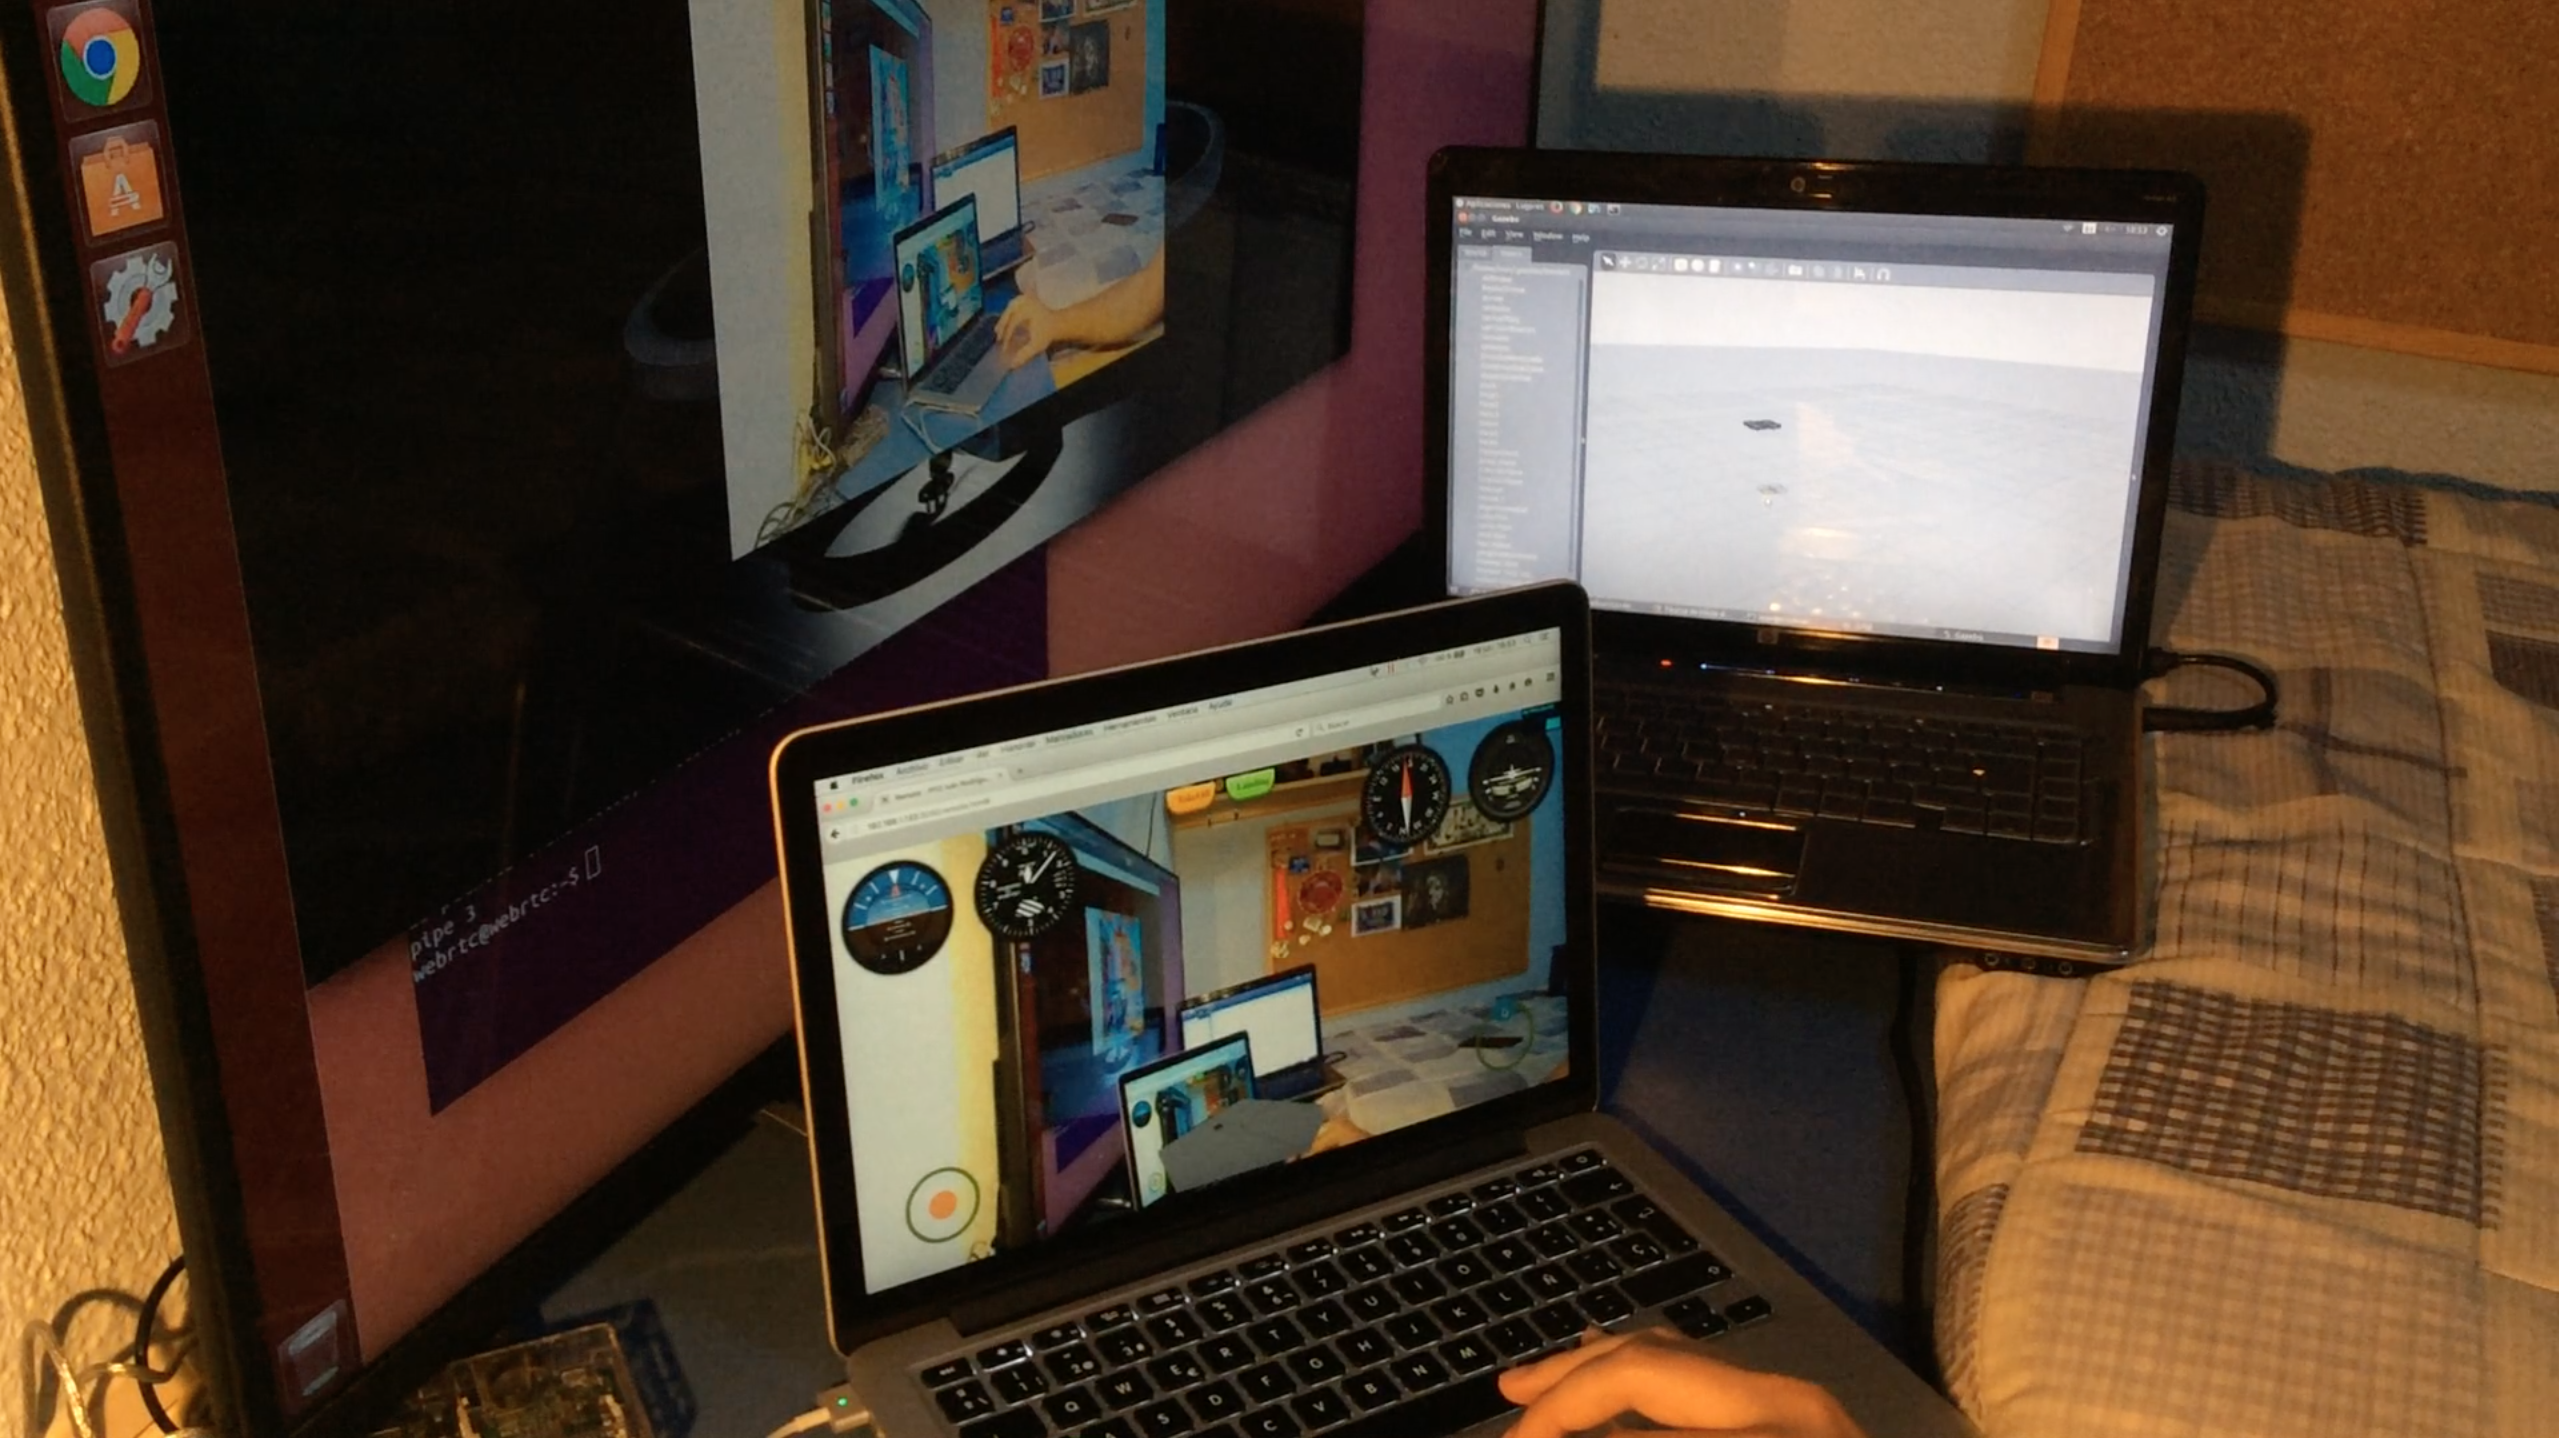
\includegraphics[width=0.9\textwidth]{experimentogazebo}
\caption{Experimento con el simulador Gazebo.}
\label{fig:experimentogazebo}
\end{figure}

En la siguiente figura (\ref{fig:secexp1}) se puede observar la secuencia de movimiento del drone durante el experimento.\\

\newpage
\begin{figure}[h!]
\centering
  \begin{subfigure}[]{47mm}
    \includegraphics[width=47mm]{sec_exp1_1}
  \end{subfigure}
  \hspace{0.5pt}
  \begin{subfigure}[]{47mm}
    \includegraphics[width=47mm]{sec_exp1_2}
  \end{subfigure}
    \hspace{0.5pt}
    \begin{subfigure}[]{47mm}
    \includegraphics[width=47mm]{sec_exp1_3}
  \end{subfigure}
    \caption{Secuencia de movimiento del drone dentro de Gazebo.}
  \label{fig:secexp1}
\end{figure}


\section{Vuelo del drone real}

Las pruebas con el drone real se han divido a su vez en dos. La primera consiste en realizar las pruebas sin colocar a bordo del drone ni el \emph{computer stick} ni la cámara. Ambos se han usado para las pruebas pero para una primera aproximación se han realizado sin estar a bordo.\\

\begin{figure}[h!]
\centering
\includegraphics[width=0.9\textwidth]{esquema_experimento2}
\caption{Esquema del experimento con el drone real.}
\label{fig:esquemaexperimento2}
\end{figure}

Así pues la distribución de los equipos es como se muestra en la figura \ref{fig:esquemaexperimento2}: computer stick como par local, que se conecta al drone real y accede a la cámara USB conectada al mismo, y ordenador portátil como par remoto desde el que se teleoperará el drone y a su vez está ejecutando el servidor de señalización y el \texttt{ardrone\_server.}\\

La figura \ref{fig:experimentodronereal1} muestra la realización de este experimento. En la mediawiki\footnote{\url{http://jderobot.org/Irodmar-tfg\#First\_Flying\_with\_Real\_Drone}}\cite{Mediawiki} hay un vídeo completo del mismo. En la figura \ref{fig:secexp2} se ha representado con tres imágenes la secuencia de vuelo del drone durante el experimento.\\

\begin{figure}[h!]
\centering
\includegraphics[width=0.9\textwidth]{experimentodronereal1}
\caption{Experimento uno con drone real.}
\label{fig:experimentodronereal1}
\end{figure}


\begin{figure}[h!]
\centering
  \begin{subfigure}[]{48mm}
    \includegraphics[width=48mm]{sec_exp2_1}
  \end{subfigure}
  \hspace{1pt}
  \begin{subfigure}[]{48mm}
    \includegraphics[width=48mm]{sec_exp2_2}
  \end{subfigure}
    \hspace{1pt}
    \begin{subfigure}[]{48mm}
    \includegraphics[width=48mm]{sec_exp2_3}
  \end{subfigure}
    \caption{Secuencia de movimiento del experimento con el drone real.}
  \label{fig:secexp2}
\end{figure}


Esta prueba también ha sido un éxito, por lo que nos marcamos el siguiente experimento con el \emph{computer stick} y la cámara a bordo del drone. Este experimento la configuración es la misma que en el anterior, pero el manejo del drone con la aplicación será más realista ya que tenemos la cámara en primera persona.\\


La segunda prueba realizada ha consistido en colocar a bordo del drone la cámara, el \emph{computer stick}, el cuál actuará como par local, estableciendo la conexión con el drone y accediendo a la cámara. El drone tiene una conexion USB de salida pero la potencia no es suficiente para hacer funcionar el \emph{computer stick}. Por este motivo se ha tenido que colocar a bordo una pila adicional la cual hará las veces de fuente de alimentación. Por otro lado tenemos un ordenador el cuál actúa como par remoto desde el que teleoperaremos el drone y además se ha utilizado para ejecutar tanto el servidor de señalización como el servidor \emph{ardrone\_server}. La figura \ref{fig:esquemaexperimentoabordo} muestra el esquema de la configuración del experimento.\\


\begin{figure}[h!]
\centering
\includegraphics[width=0.7\textwidth]{esquema_experimento_abordo}
\caption{Esquema de la configuración del experimento.}
\label{fig:esquemaexperimentoabordo}
\end{figure}


En la figura \ref{fig:elementosabordo} se muestra la configuración de todos los elementos que hemos colocado a bordo del drone. Como se puede observar también hemos incluido un hub USB ya que es necesario al disponer el \emph{computer stick} de un único puerto USB y necesitar al menos dos, uno para la cámara y otro para el ratón en el momento que configuramos el navegador. Puede ver el montaje final en este vídeo\footnote{\url{http://jderobot.org/Irodmar-tfg#Experiment_Setup}} de la mediawiki.\\

\begin{figure}[h!]
\centering
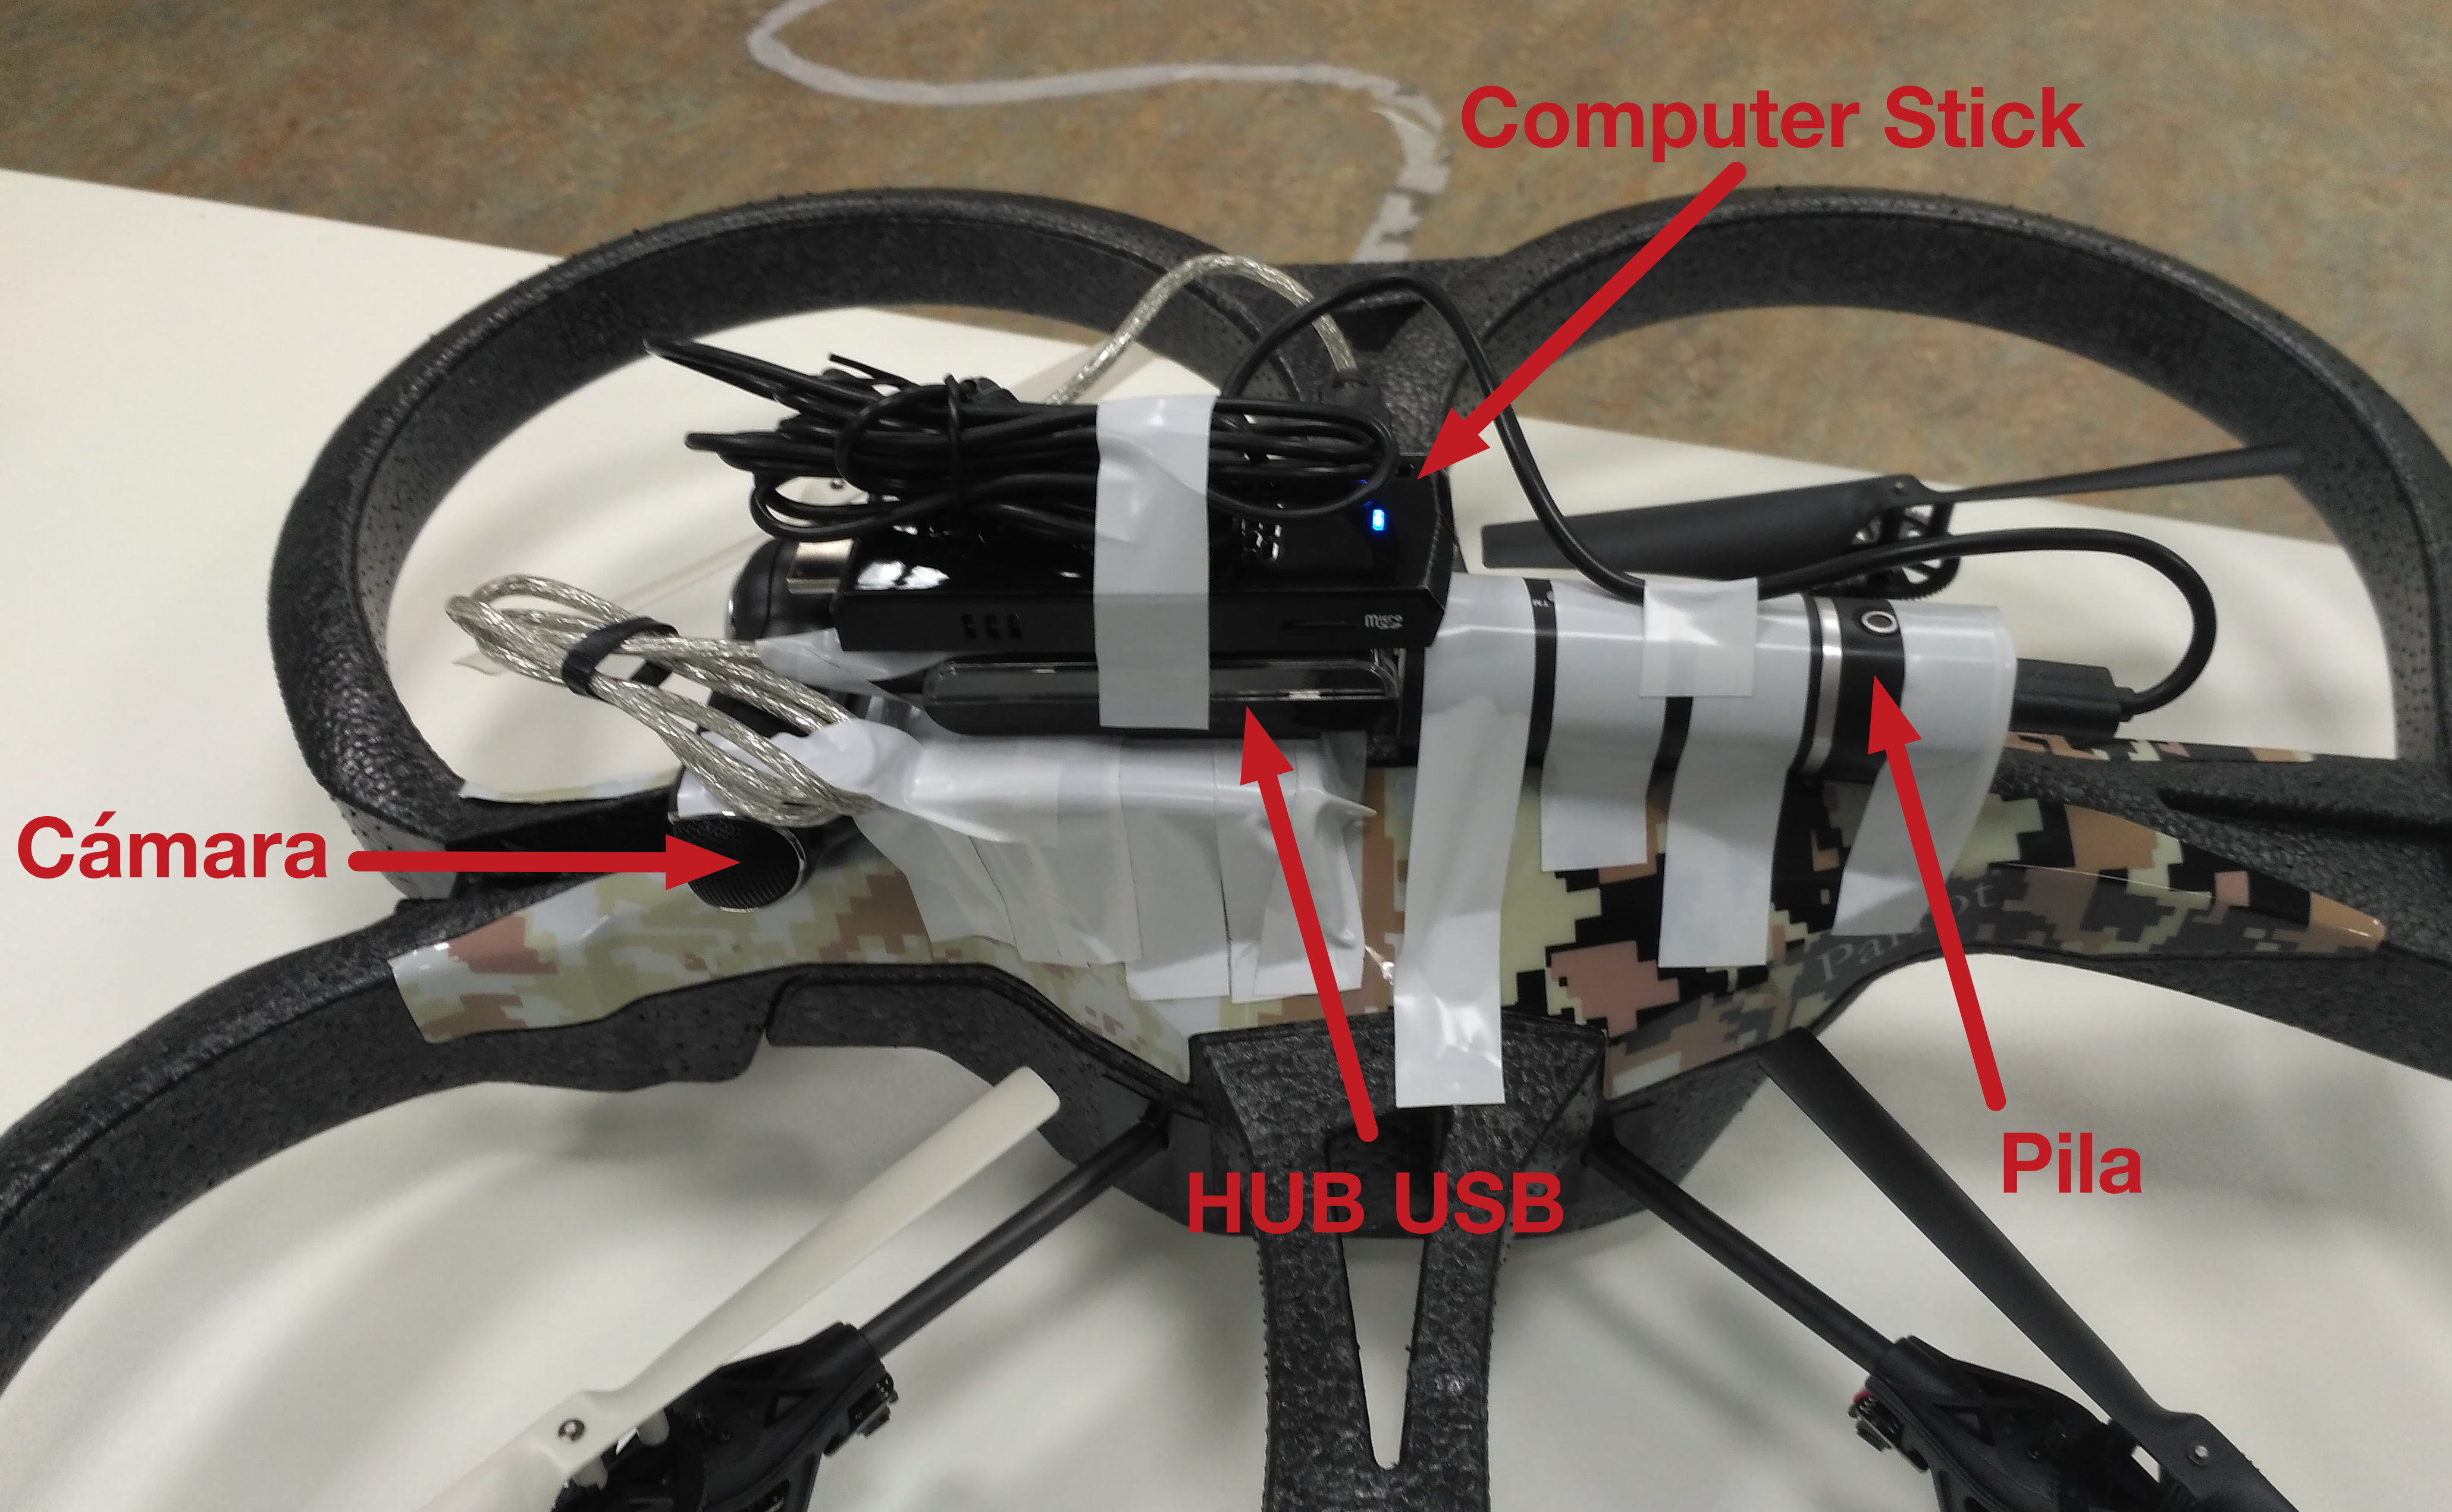
\includegraphics[width=0.8\textwidth]{elementos_abordo}
\caption{Configuración de los elementos a bordo del drone.}
\label{fig:elementosabordo}
\end{figure}


Este experimento ha sido fallido, únicamente por las capacidades de vuelo que nos ofrece el drone. Entre los dispositivos que hemos colocado a bordo superamos la carga máxima de pago que permite este cuadricóptero. En lo que al funcionamiento de la aplicación se refiere ha funcionado perfectamente ya que en el par remoto obteníamos las imágenes y datos de vuelo procedentes del drone, y al ejecutar la orden de despegue el cuadricóptero ha intentado levantar el vuelo sin conseguirlo.\\

\begin{figure}[h!]
\centering
\includegraphics[width=0.7\textwidth]{experimento_abordo}
\caption{ArDrone no levanta el vuelo por exceso de peso.}
\label{fig:experimentoabordo}
\end{figure}

La figura \ref{fig:experimentoabordo} es un fotográma del vídeo\footnote{\url{http://jderobot.org/Irodmar-tfg#Attemp_of_flying}} que se grabó durante el experimento. En ella se ve al drone intentando levantar el vuelo. Para comprobar que el desarrollo funciona se optó por realizar otra prueba de vuelo en la que se cogía con las manos el drone y se le movía para observar que tanto la cámara a bordo cómo los relojes de vuelo variaban en el navegador remoto. La figura \ref{fig:pruebaexperimentoabordo} muestra un fotograma del vídeo\footnote{\url{http://jderobot.org/Irodmar-tfg#Testing_the_development}} en el que se realizan estas comprobaciones.\\

\begin{figure}[h!]
\centering
\includegraphics[width=0.7\textwidth]{pruebas_experimento_abordo}
\caption{Comprobación del funcionamiento de la aplicación.}
\label{fig:pruebaexperimentoabordo}
\end{figure}

\section{Vuelos con multidispositivos}

Como tercer y último experimento hemos probado a volar el drone utilizando dispositivos móviles. WebRTC tiene soporte para dispositivos móviles y los elementos de control los hemos desarrollado también para dispositivos táctiles, podemos utilizarlos como par remoto, par local o ambos. Al igual que el experimento anterior se ha realizado en dos pasos. Primero sin colocar el dispositivo a bordo del drone para confirmar su correcto funcionamiento y posteriormente repitiéndolo con el dispositivo a bordo. Realizar experimentos con dispositivos móviles implica la necesidad de la utilización de un ordenador de apoyo que será el que ejecute tanto el servidor de señalización para WebRTC cómo \texttt{ardrone\_server}.\\


\begin{figure}[h!]
\centering
\includegraphics[width=0.8\textwidth]{esquema_experimento_multidispositivo_1}
\caption{Esquema del experimento con móvil como par remoto.}
\label{fig:esquemaexperimentomultidispositivo}
\end{figure}


Como primer experimento se ha utilizado un ordenador portátil como par local, encargado por un lado de estableciendo la conexion con el drone y de acceder a la cámara, en este caso la incorporada en el portátil, y por otro lado de correr los servidores de señalización y \texttt{ardrone\_server}. Como par remoto para teleoperar el drone se ha utilizado un teléfono móvil. En la figura \ref{fig:esquemaexperimentomultidispositivo} se detalla el esquema de este experimento.\\


En la figura \ref{fig:experimentodronemultidispositivo1} se puede apreciar un instante del experimento cuyo vídeo se encuentra en la mediawiki\footnote{\url{http://jderobot.org/Irodmar-tfg\#Flying\_with\_a\_mobile\_like\_Remote\_PC}}. En la figura \ref{fig:secexp3} podemos ver la secuencia de movimiento del drone teleoperado con un dispositivo móvil.\\

\begin{figure}[h!]
\centering
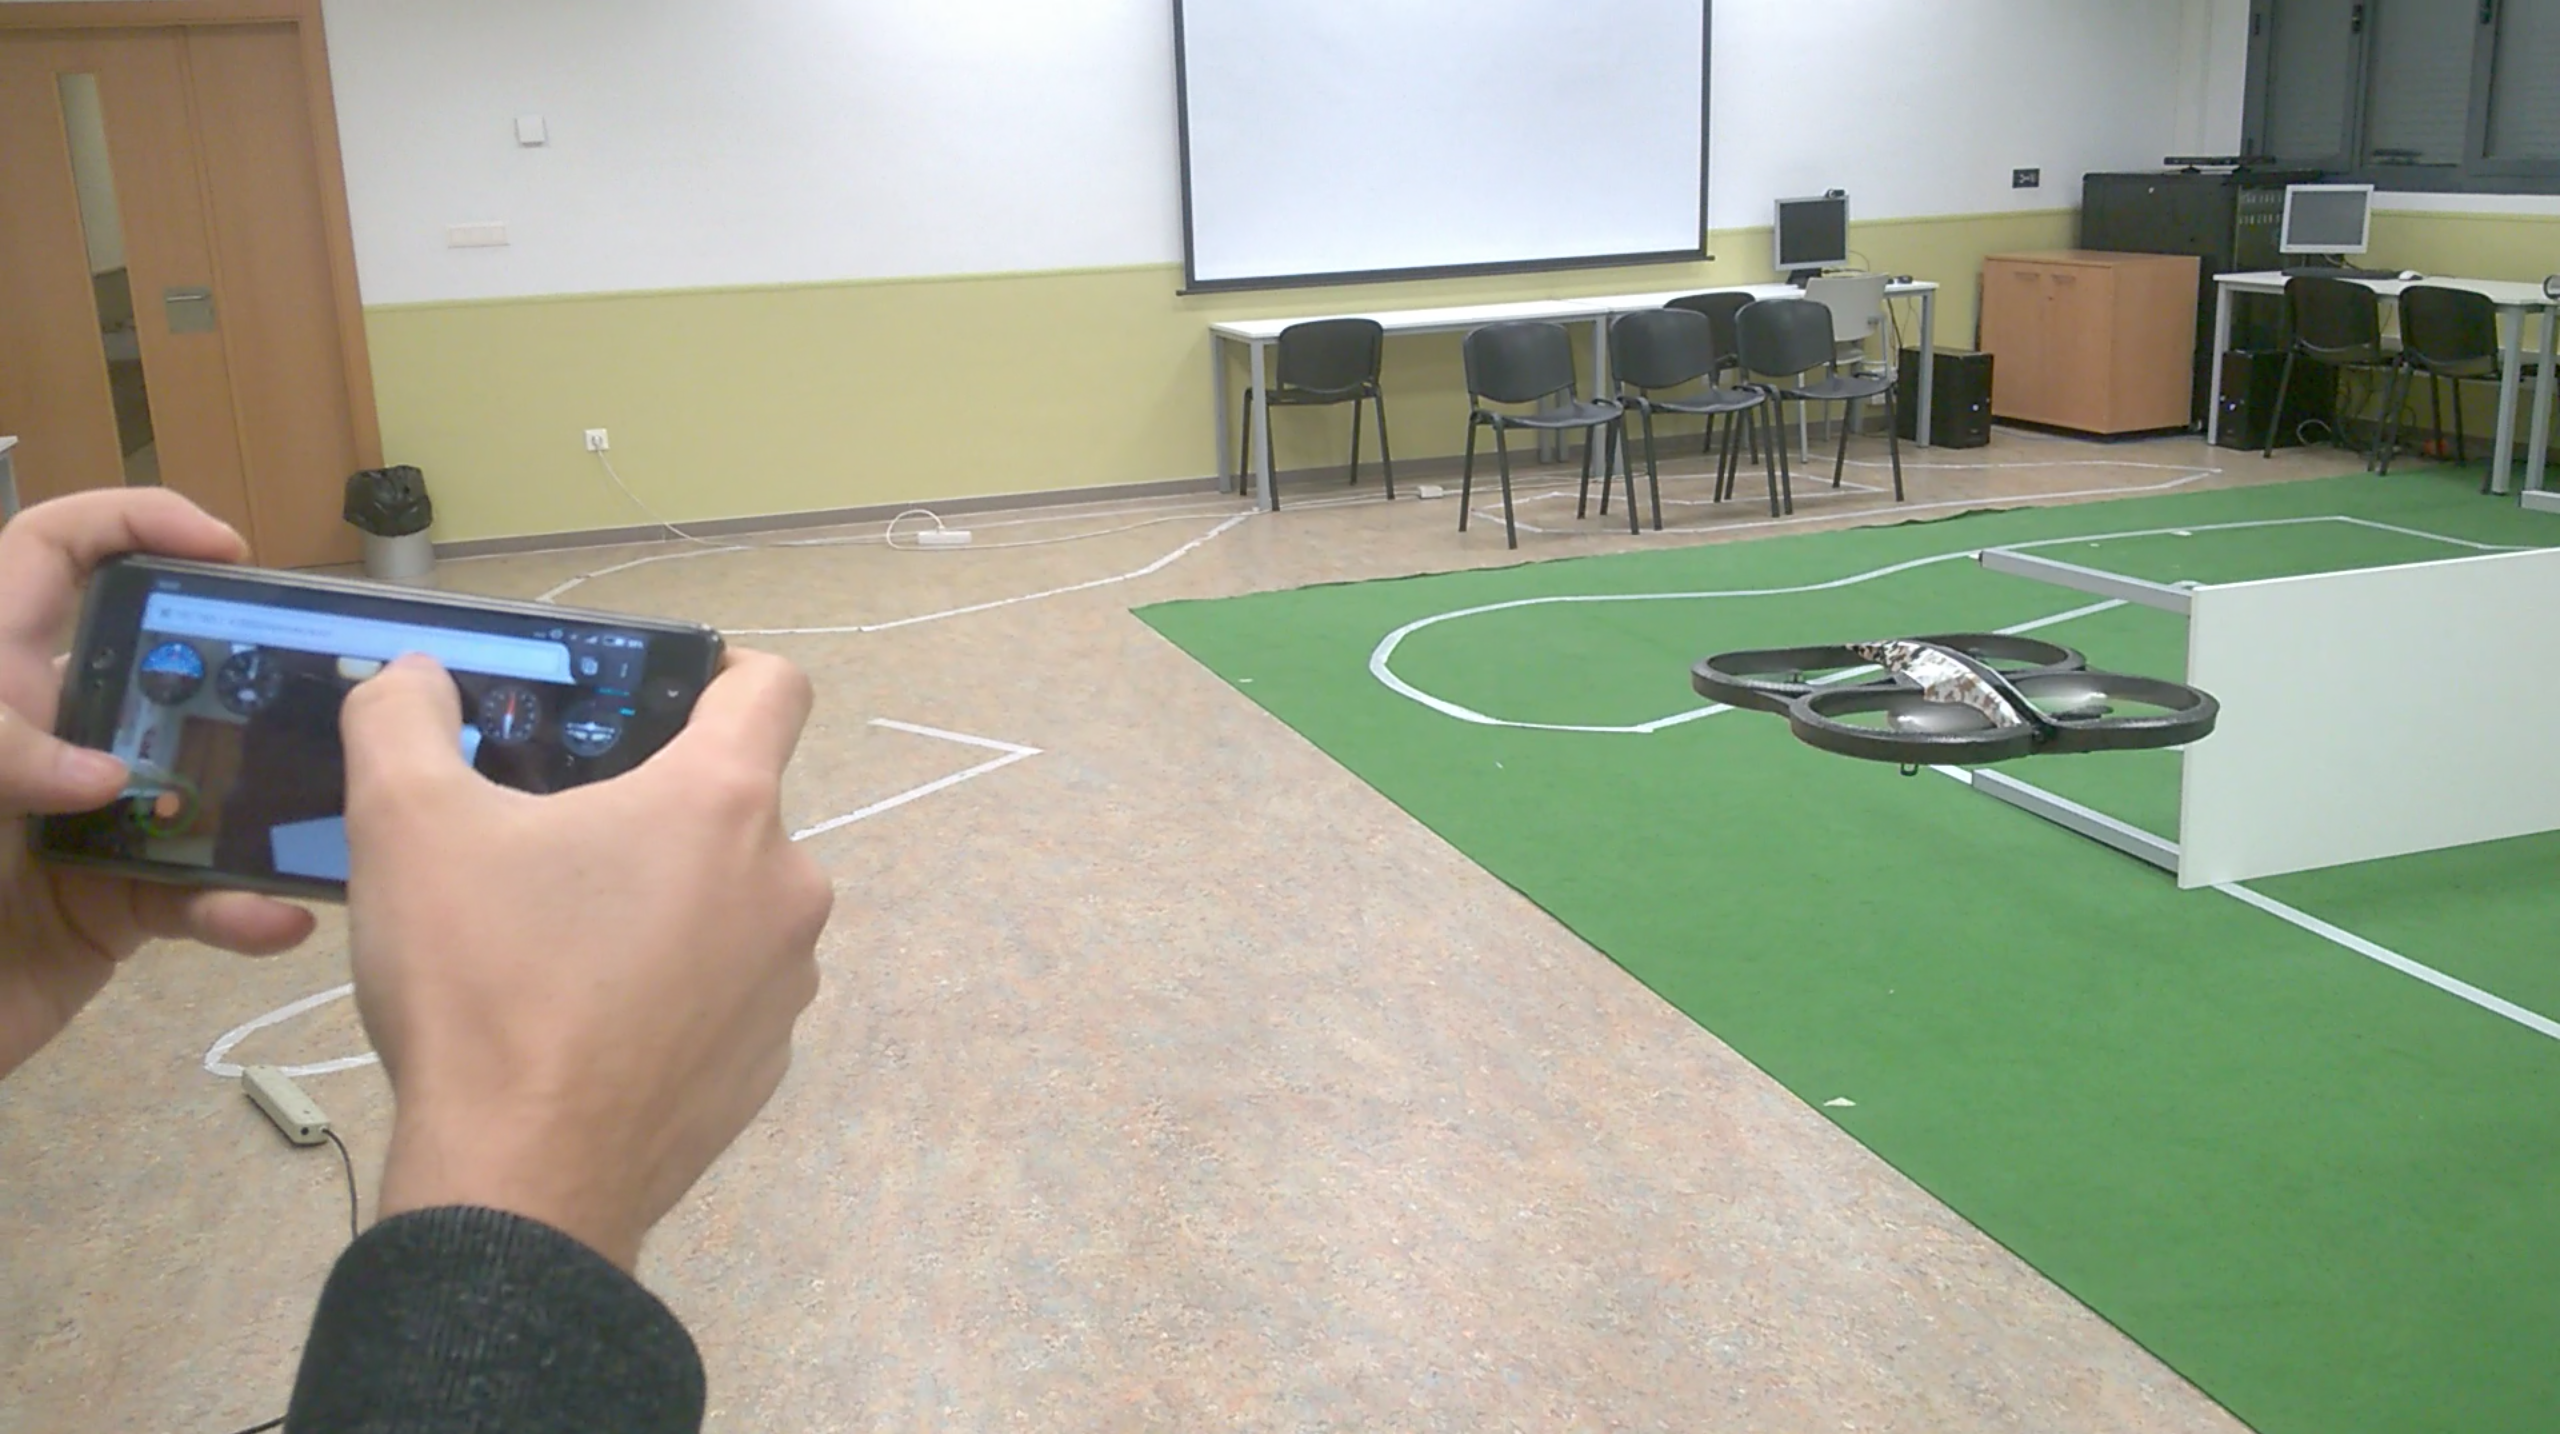
\includegraphics[width=0.9\textwidth]{experimentodronemultidispositivo1}
\caption{Experimento con móvil como par remoto.}
\label{fig:experimentodronemultidispositivo1}
\end{figure}


\begin{figure}[h!]
\centering
  \begin{subfigure}[]{48mm}
    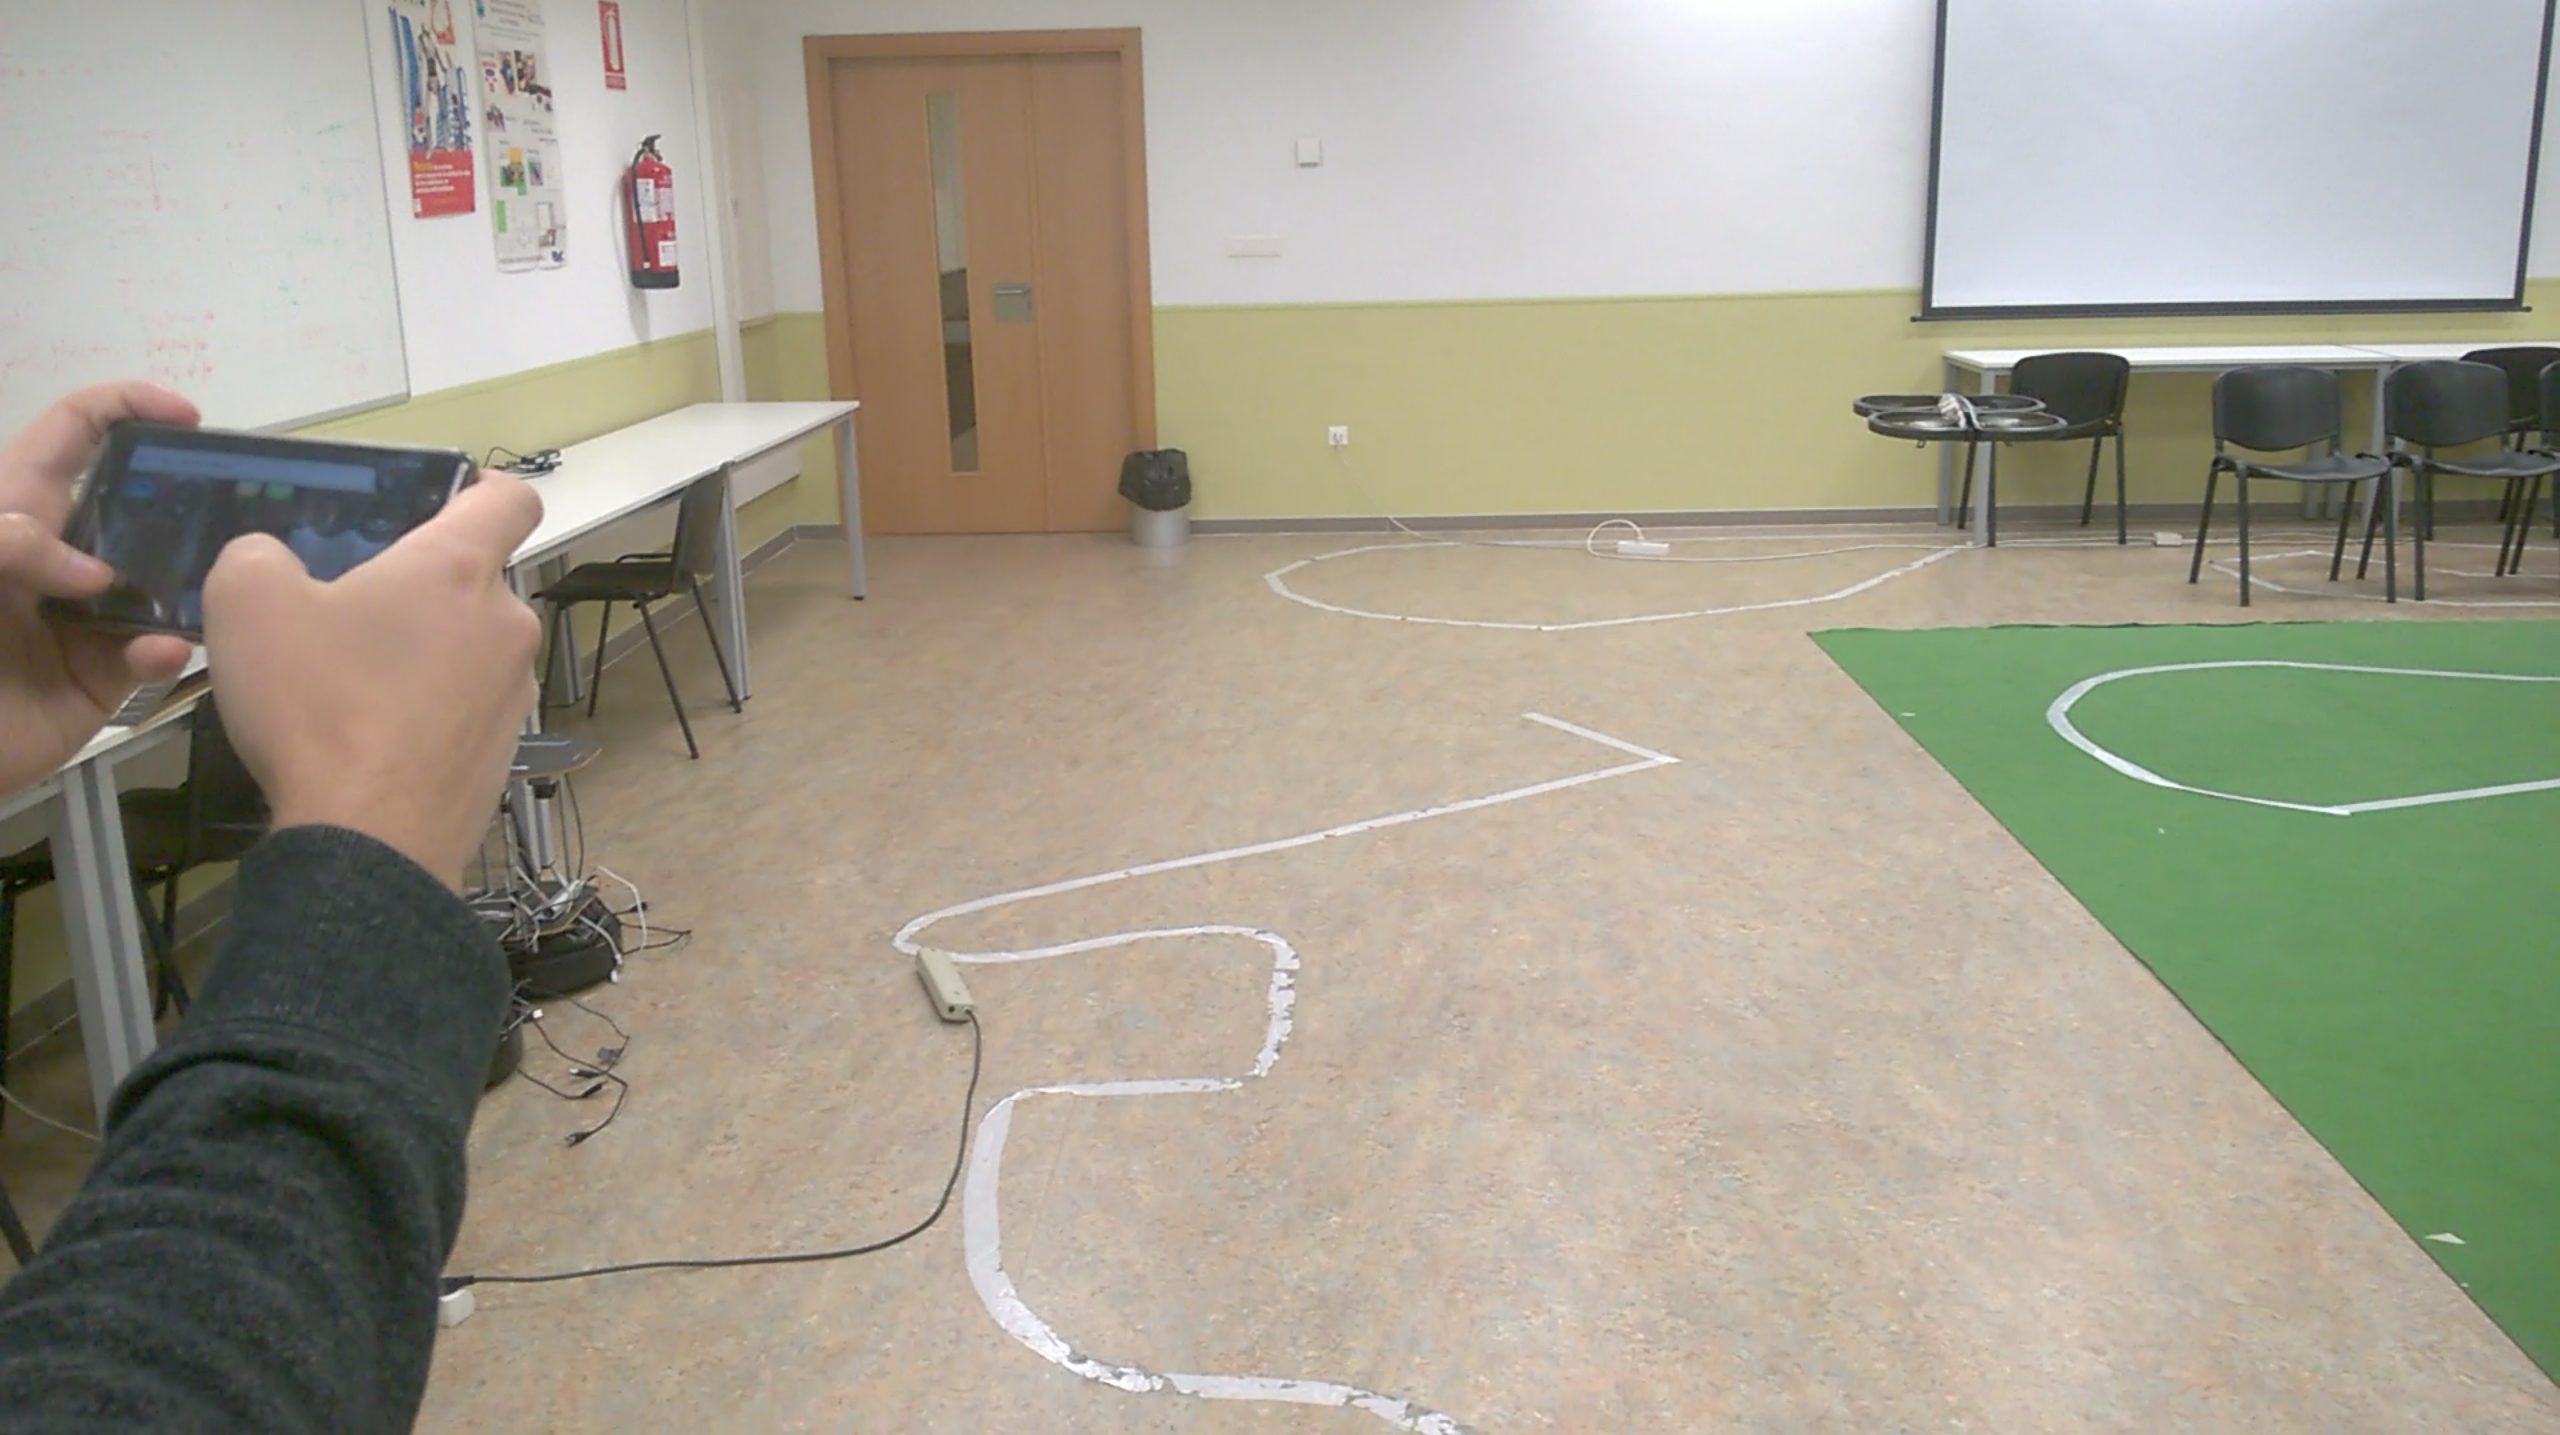
\includegraphics[width=48mm]{sec_exp3_1}
  \end{subfigure}
  \hspace{1pt}
  \begin{subfigure}[]{48mm}
    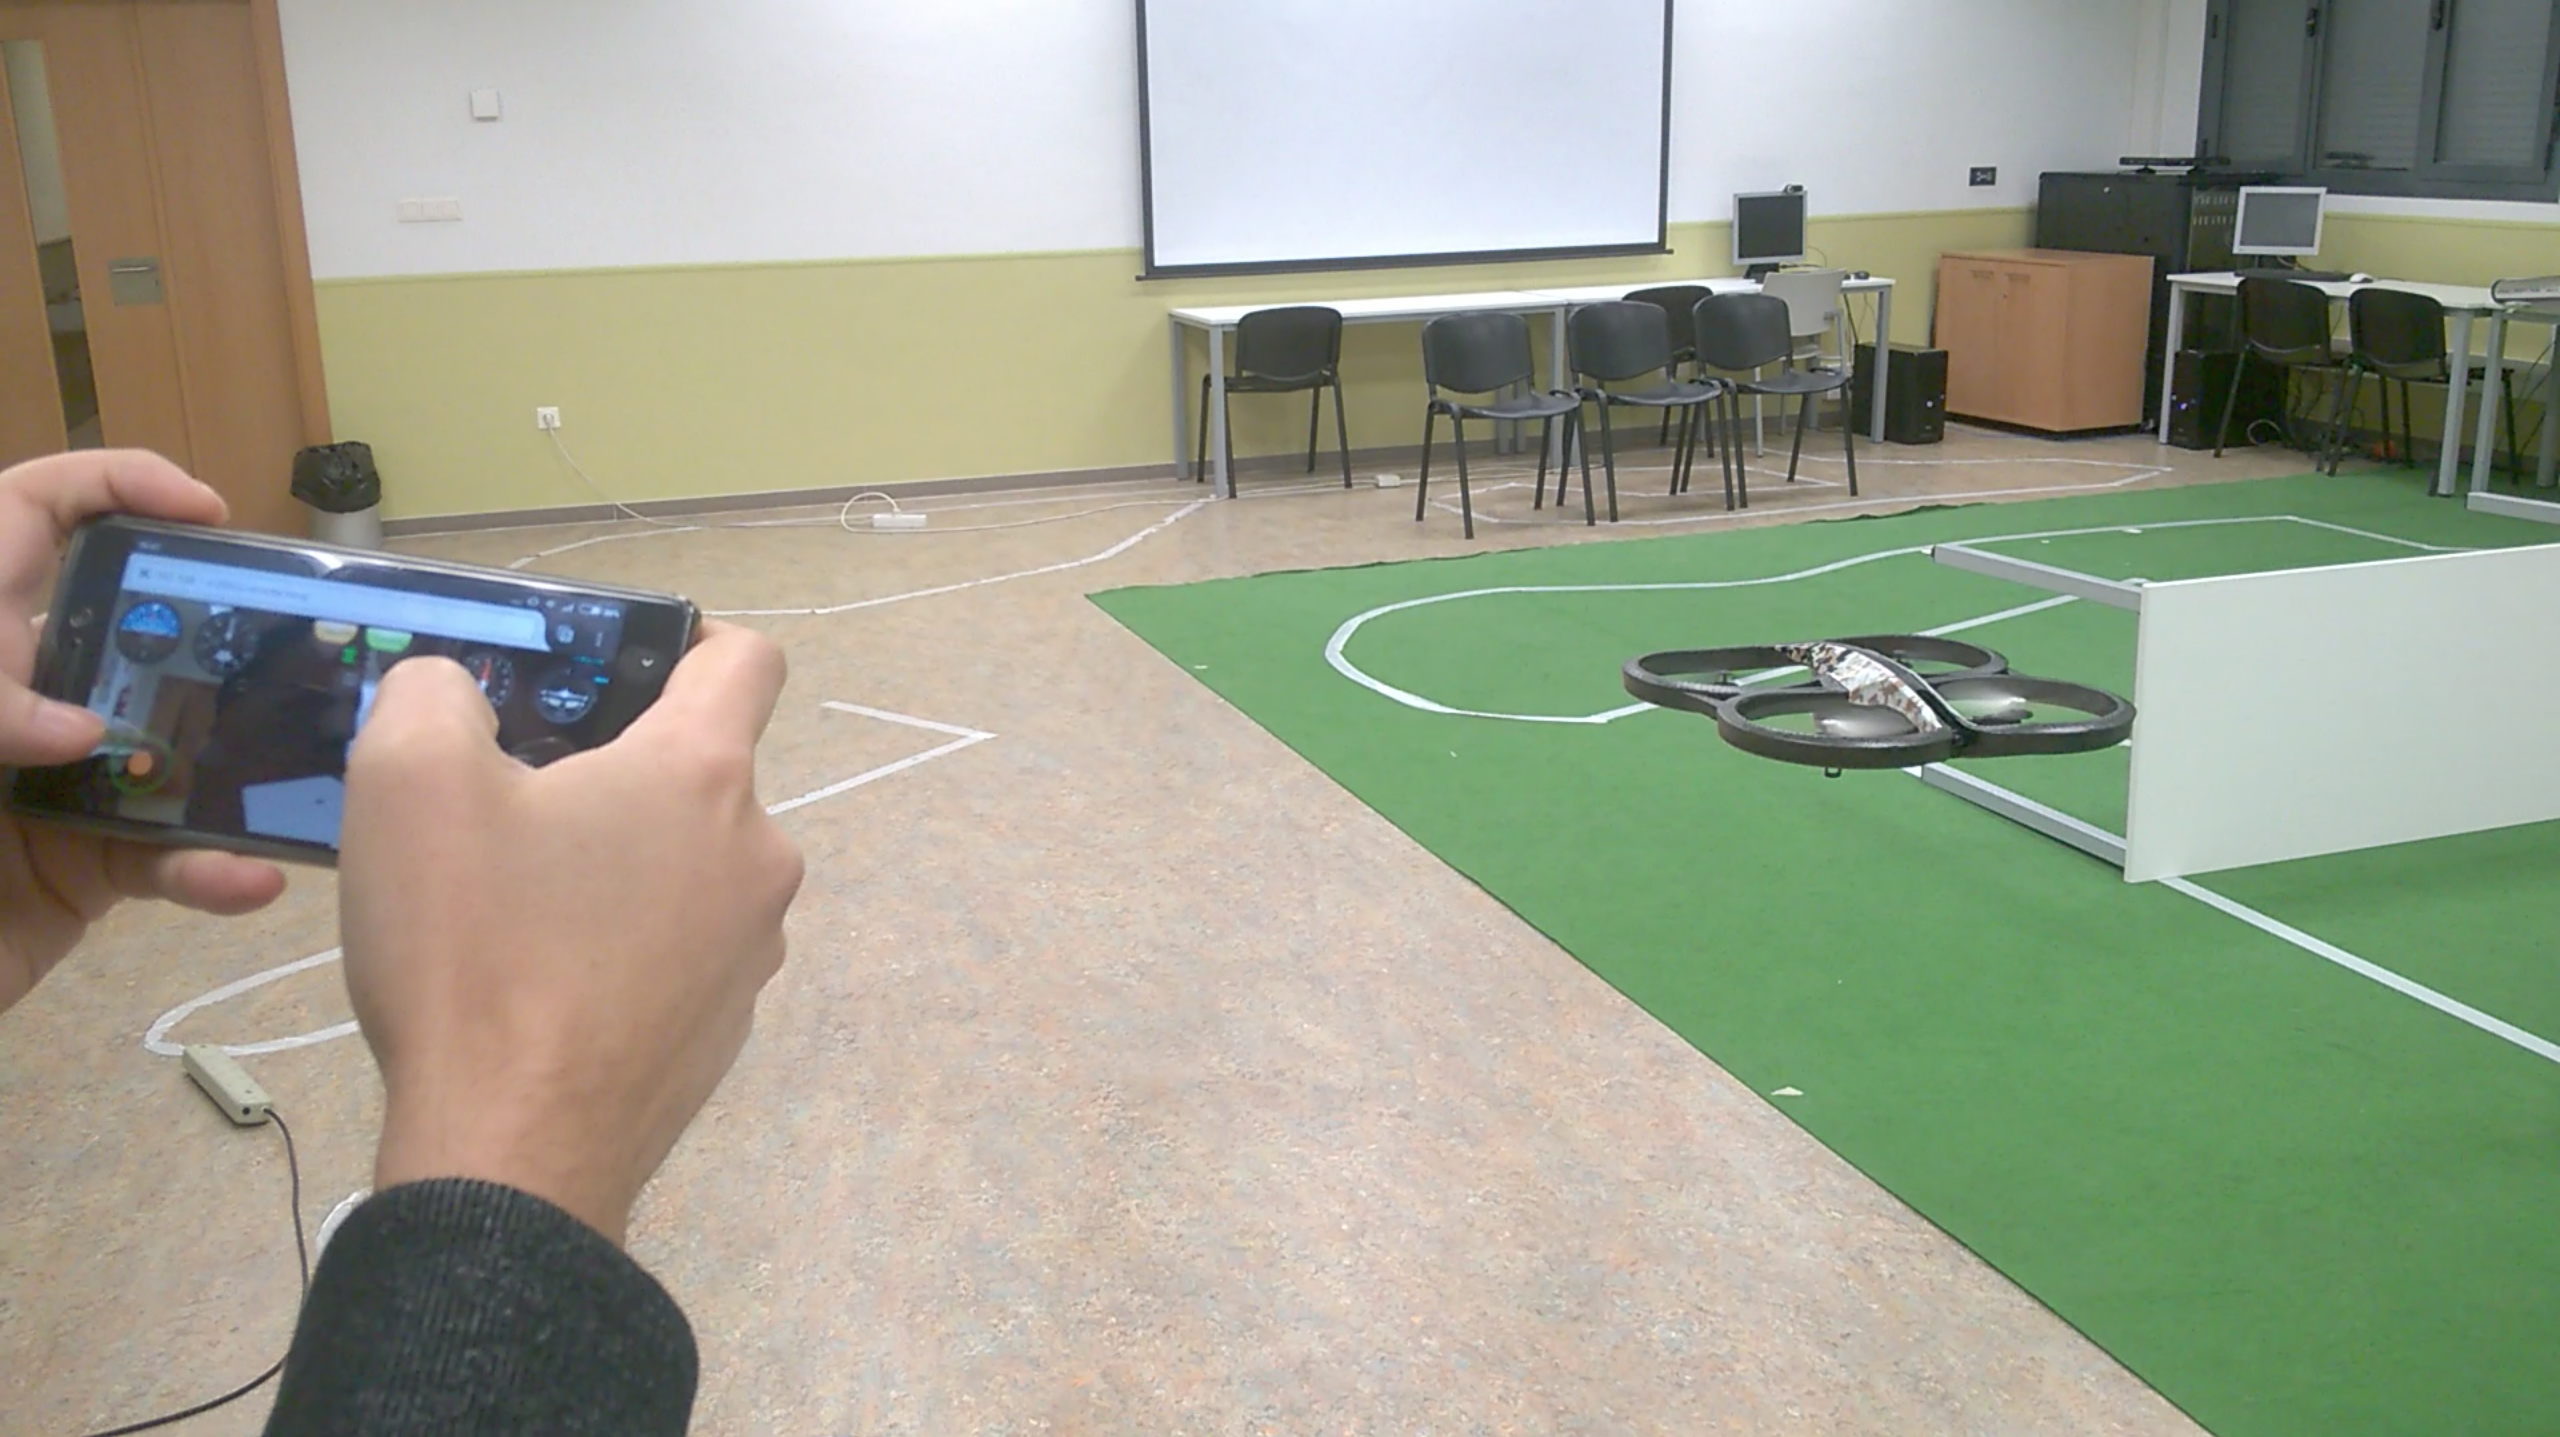
\includegraphics[width=48mm]{sec_exp3_2}
  \end{subfigure}
    \hspace{1pt}
    \begin{subfigure}[]{48mm}
    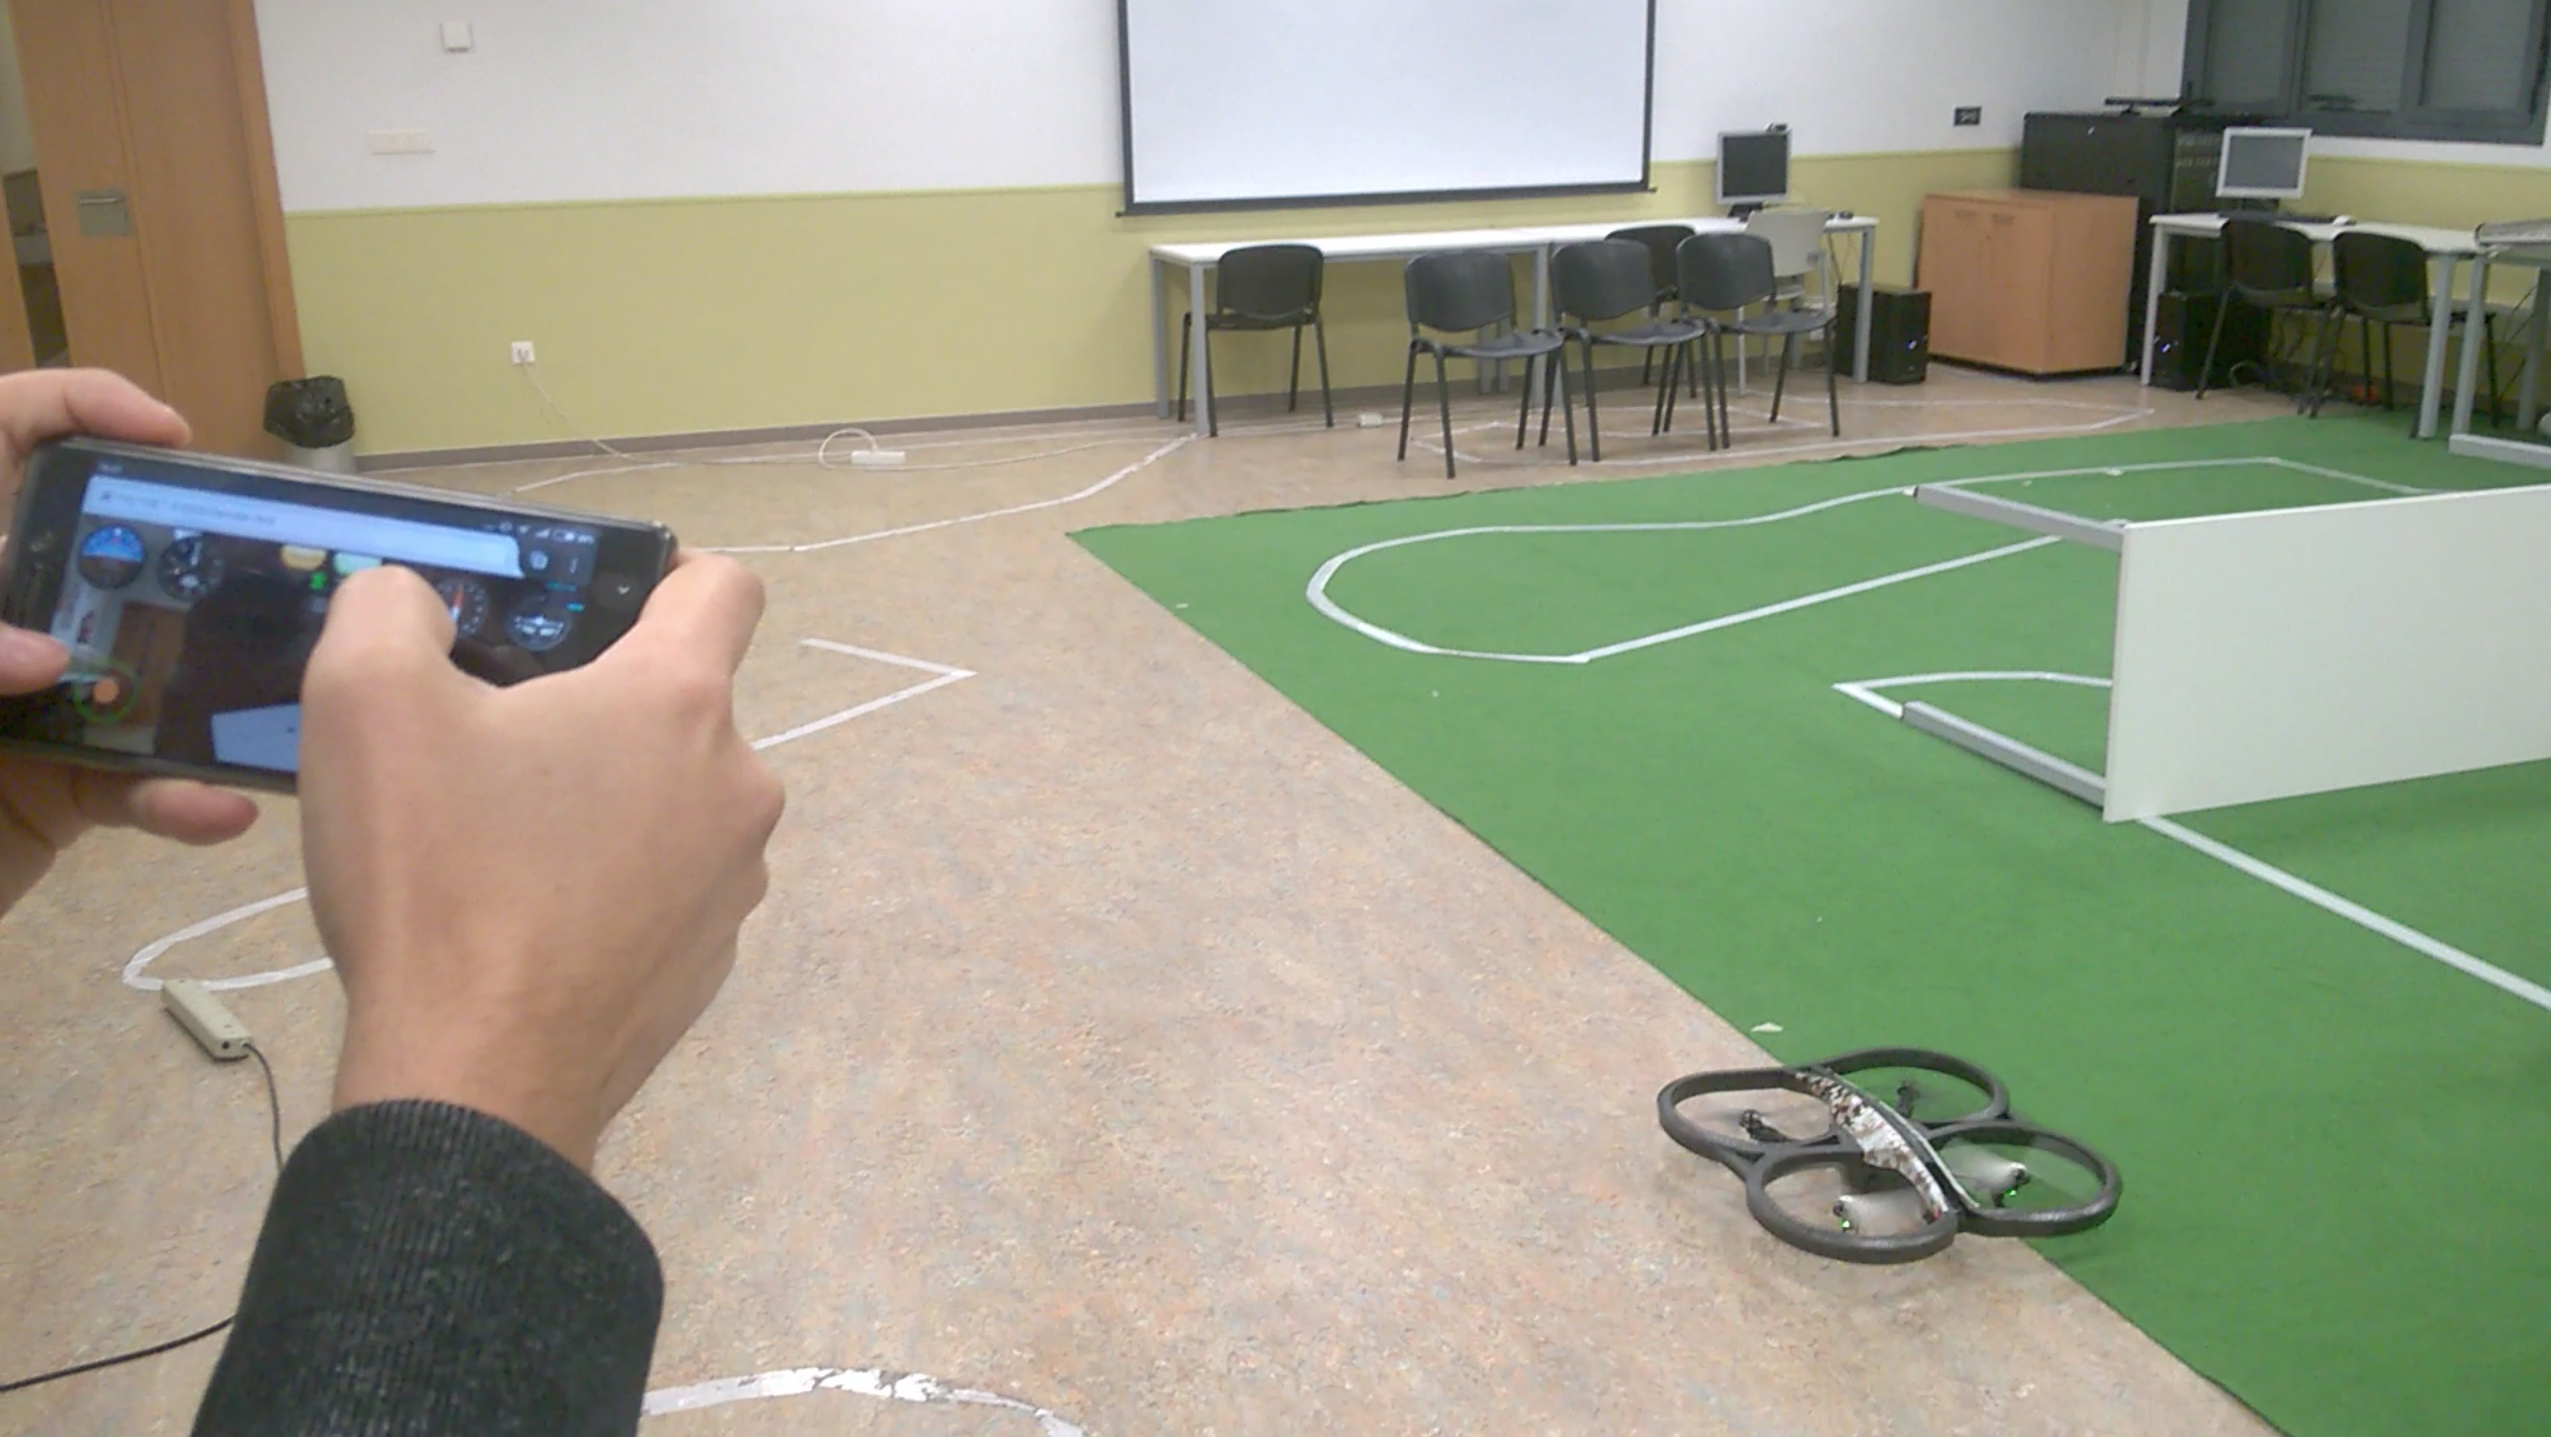
\includegraphics[width=48mm]{sec_exp3_3}
  \end{subfigure}
    \caption{Secuencia de movimiento del experimento con dispositivo móvil como par remoto.}
  \label{fig:secexp3}
\end{figure}


\newpage
El segundo experimento (figura \ref{fig:esquemaexperimentomultidispositivo2}) es a la inversa, se utiliza un ordenador portátil como par remoto y un teléfono móvil como par local.

\begin{figure}[h!]
\centering
\includegraphics[width=0.8\textwidth]{experimento_multidispositivo2}
\caption{Esquema del experimento con móvil como par local.}
\label{fig:esquemaexperimentomultidispositivo2}
\end{figure}

En este configuración el ordenador portátil se utiliza también para ejecutar los servidores de señalización y \texttt{ardrone\_server}. El móvil se usa como par local, encargándose de establecer la conexion con el drone. En este caso las imágenes que se envían son de una de las dos cámaras del móvil, la delantera o la trasera, pudiendo elegir cualquiera de las dos. En este experimento el móvil lo colocamos sobre la mesa mirando hacia la posición en la que se encuentra en drone, por lo que en la pantalla del ordenador remoto le veremos moviéndose. La figura \ref{fig:experimentodronemultidispositivo2} muestra un momento del experimento que esta recogido en un vídeo en la mediawiki\footnote{\url{http://jderobot.org/Irodmar-tfg#Flying_with_a_mobile_like_Droner_PC}}. En la figura \ref{fig:secexp4} se muestra una secuencia del vuelo realizado.\\

\begin{figure}[h!]
\centering
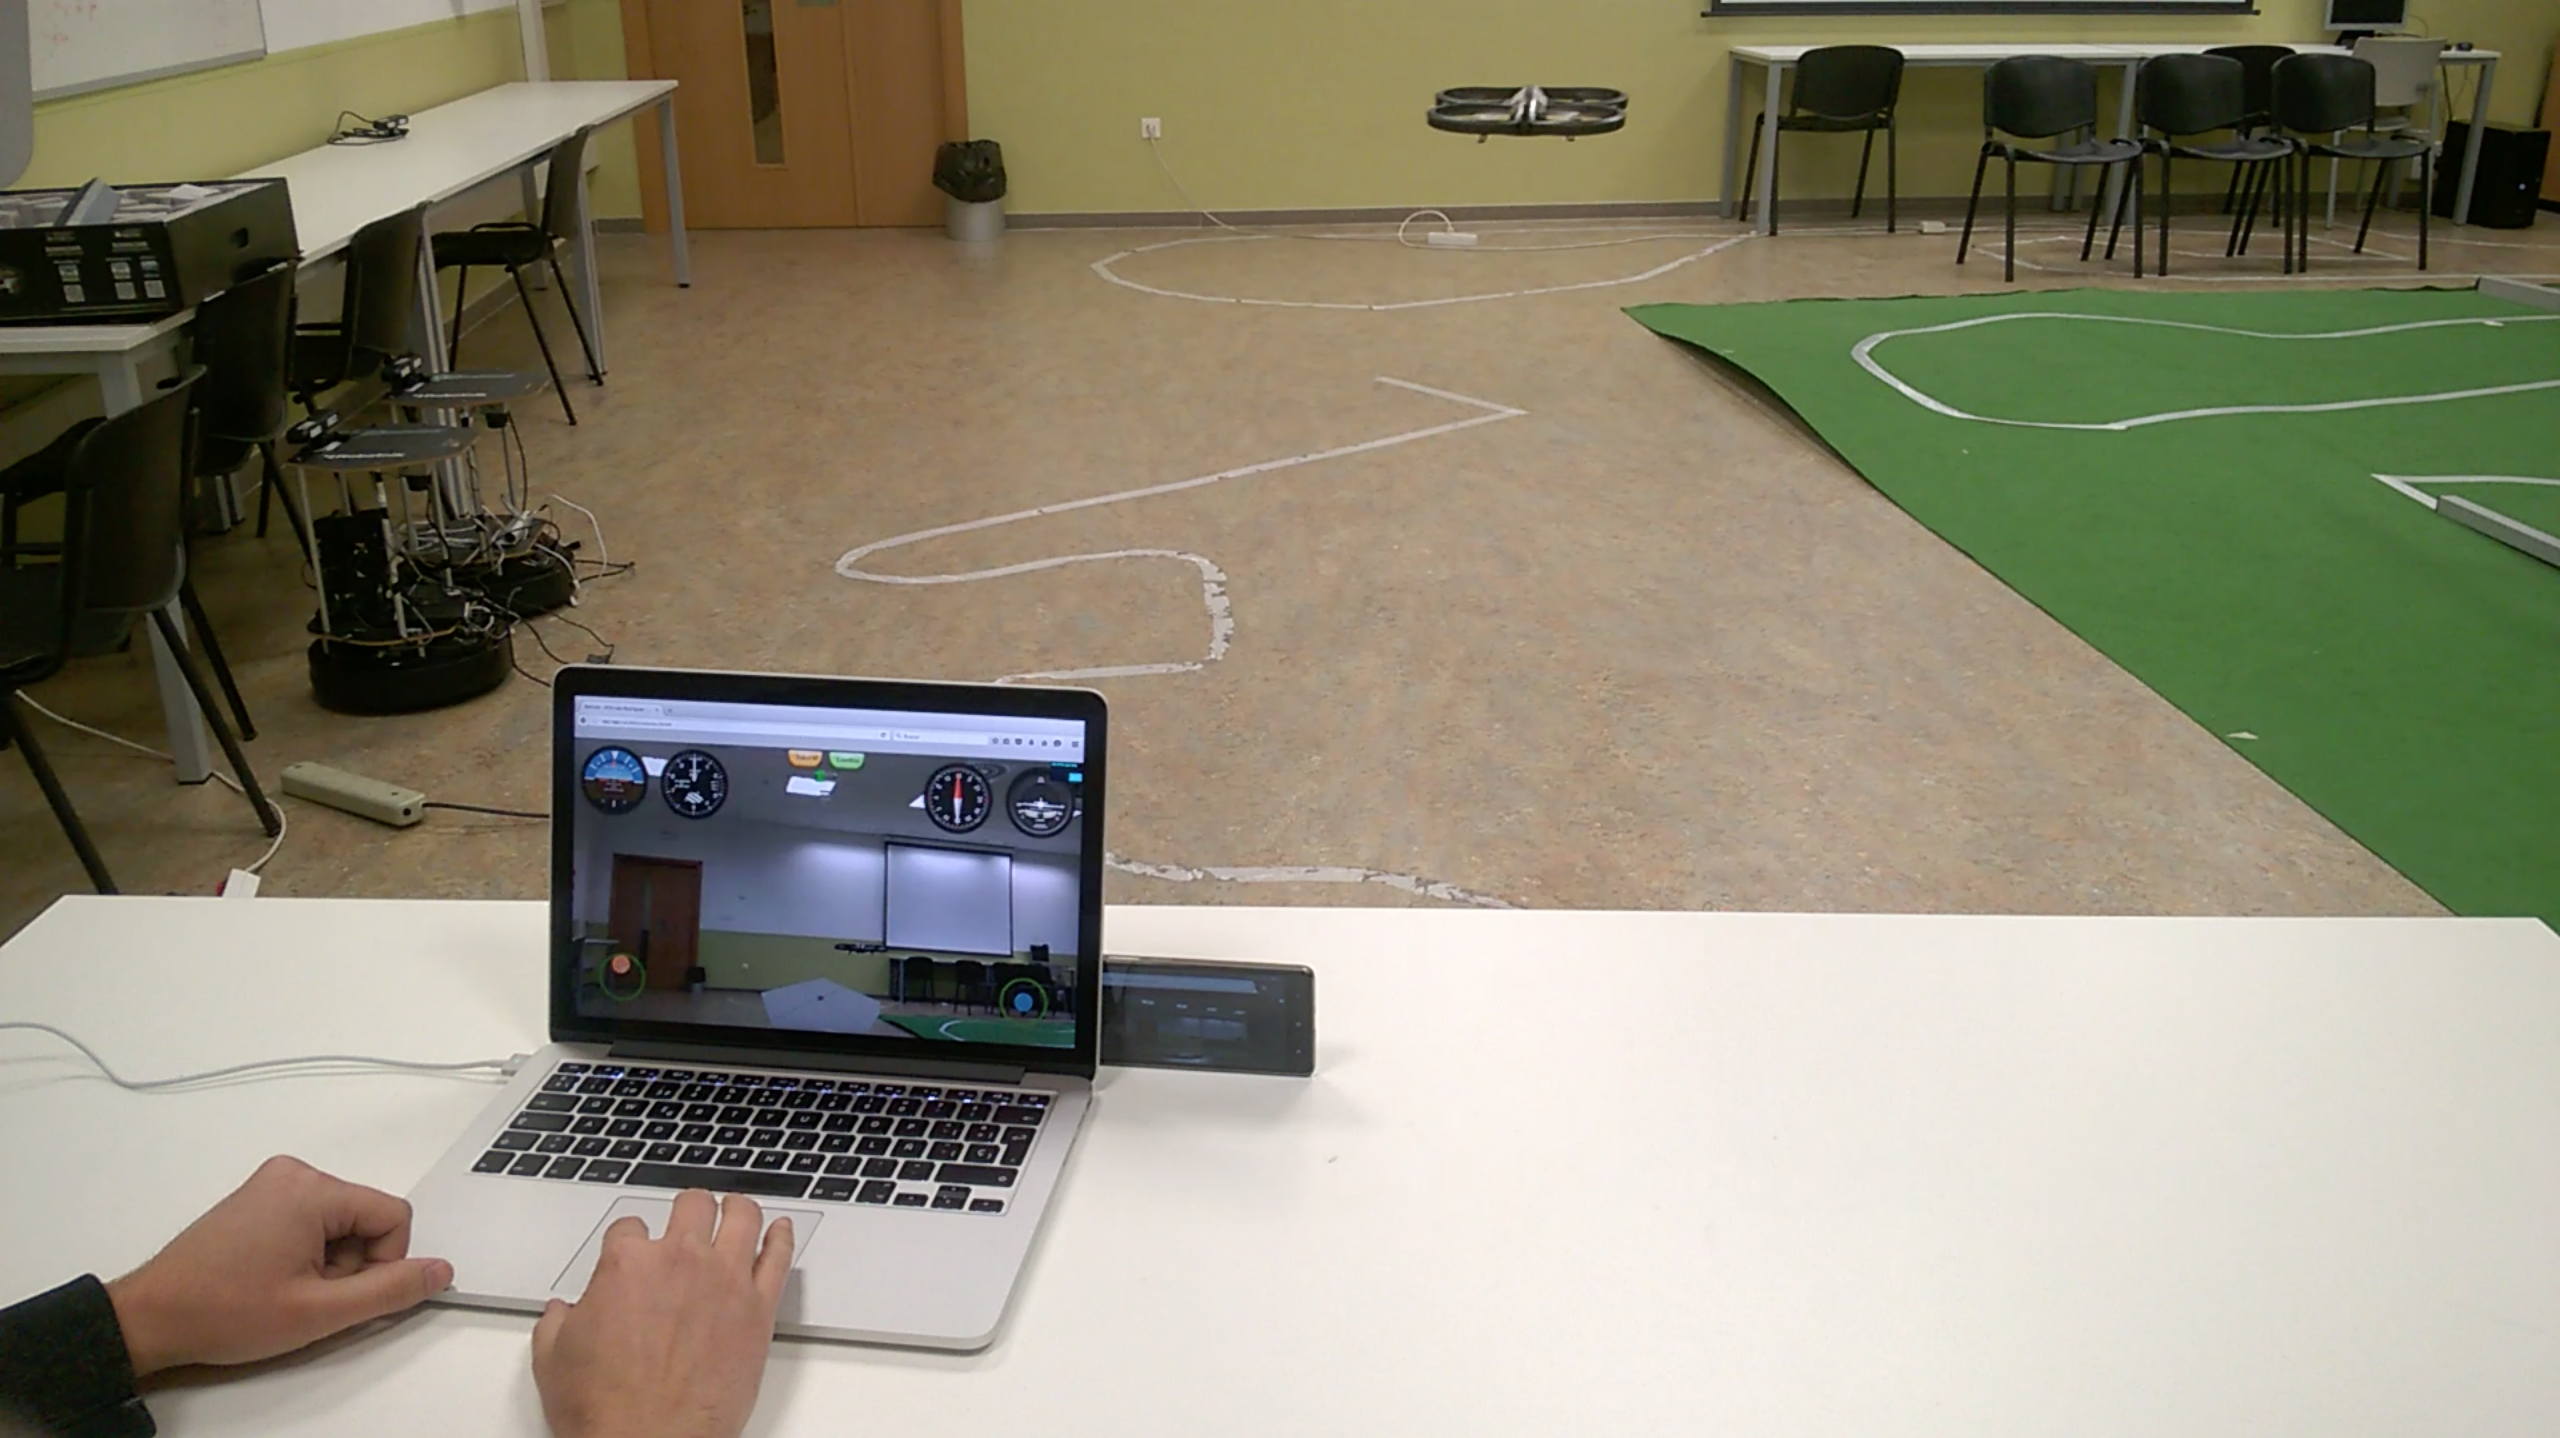
\includegraphics[width=0.9\textwidth]{experimentodronemultidispositivo2}
\caption{Experimento con móvil como par local.}
\label{fig:experimentodronemultidispositivo2}
\end{figure}


\begin{figure}[h!]
\centering
  \begin{subfigure}[]{48mm}
    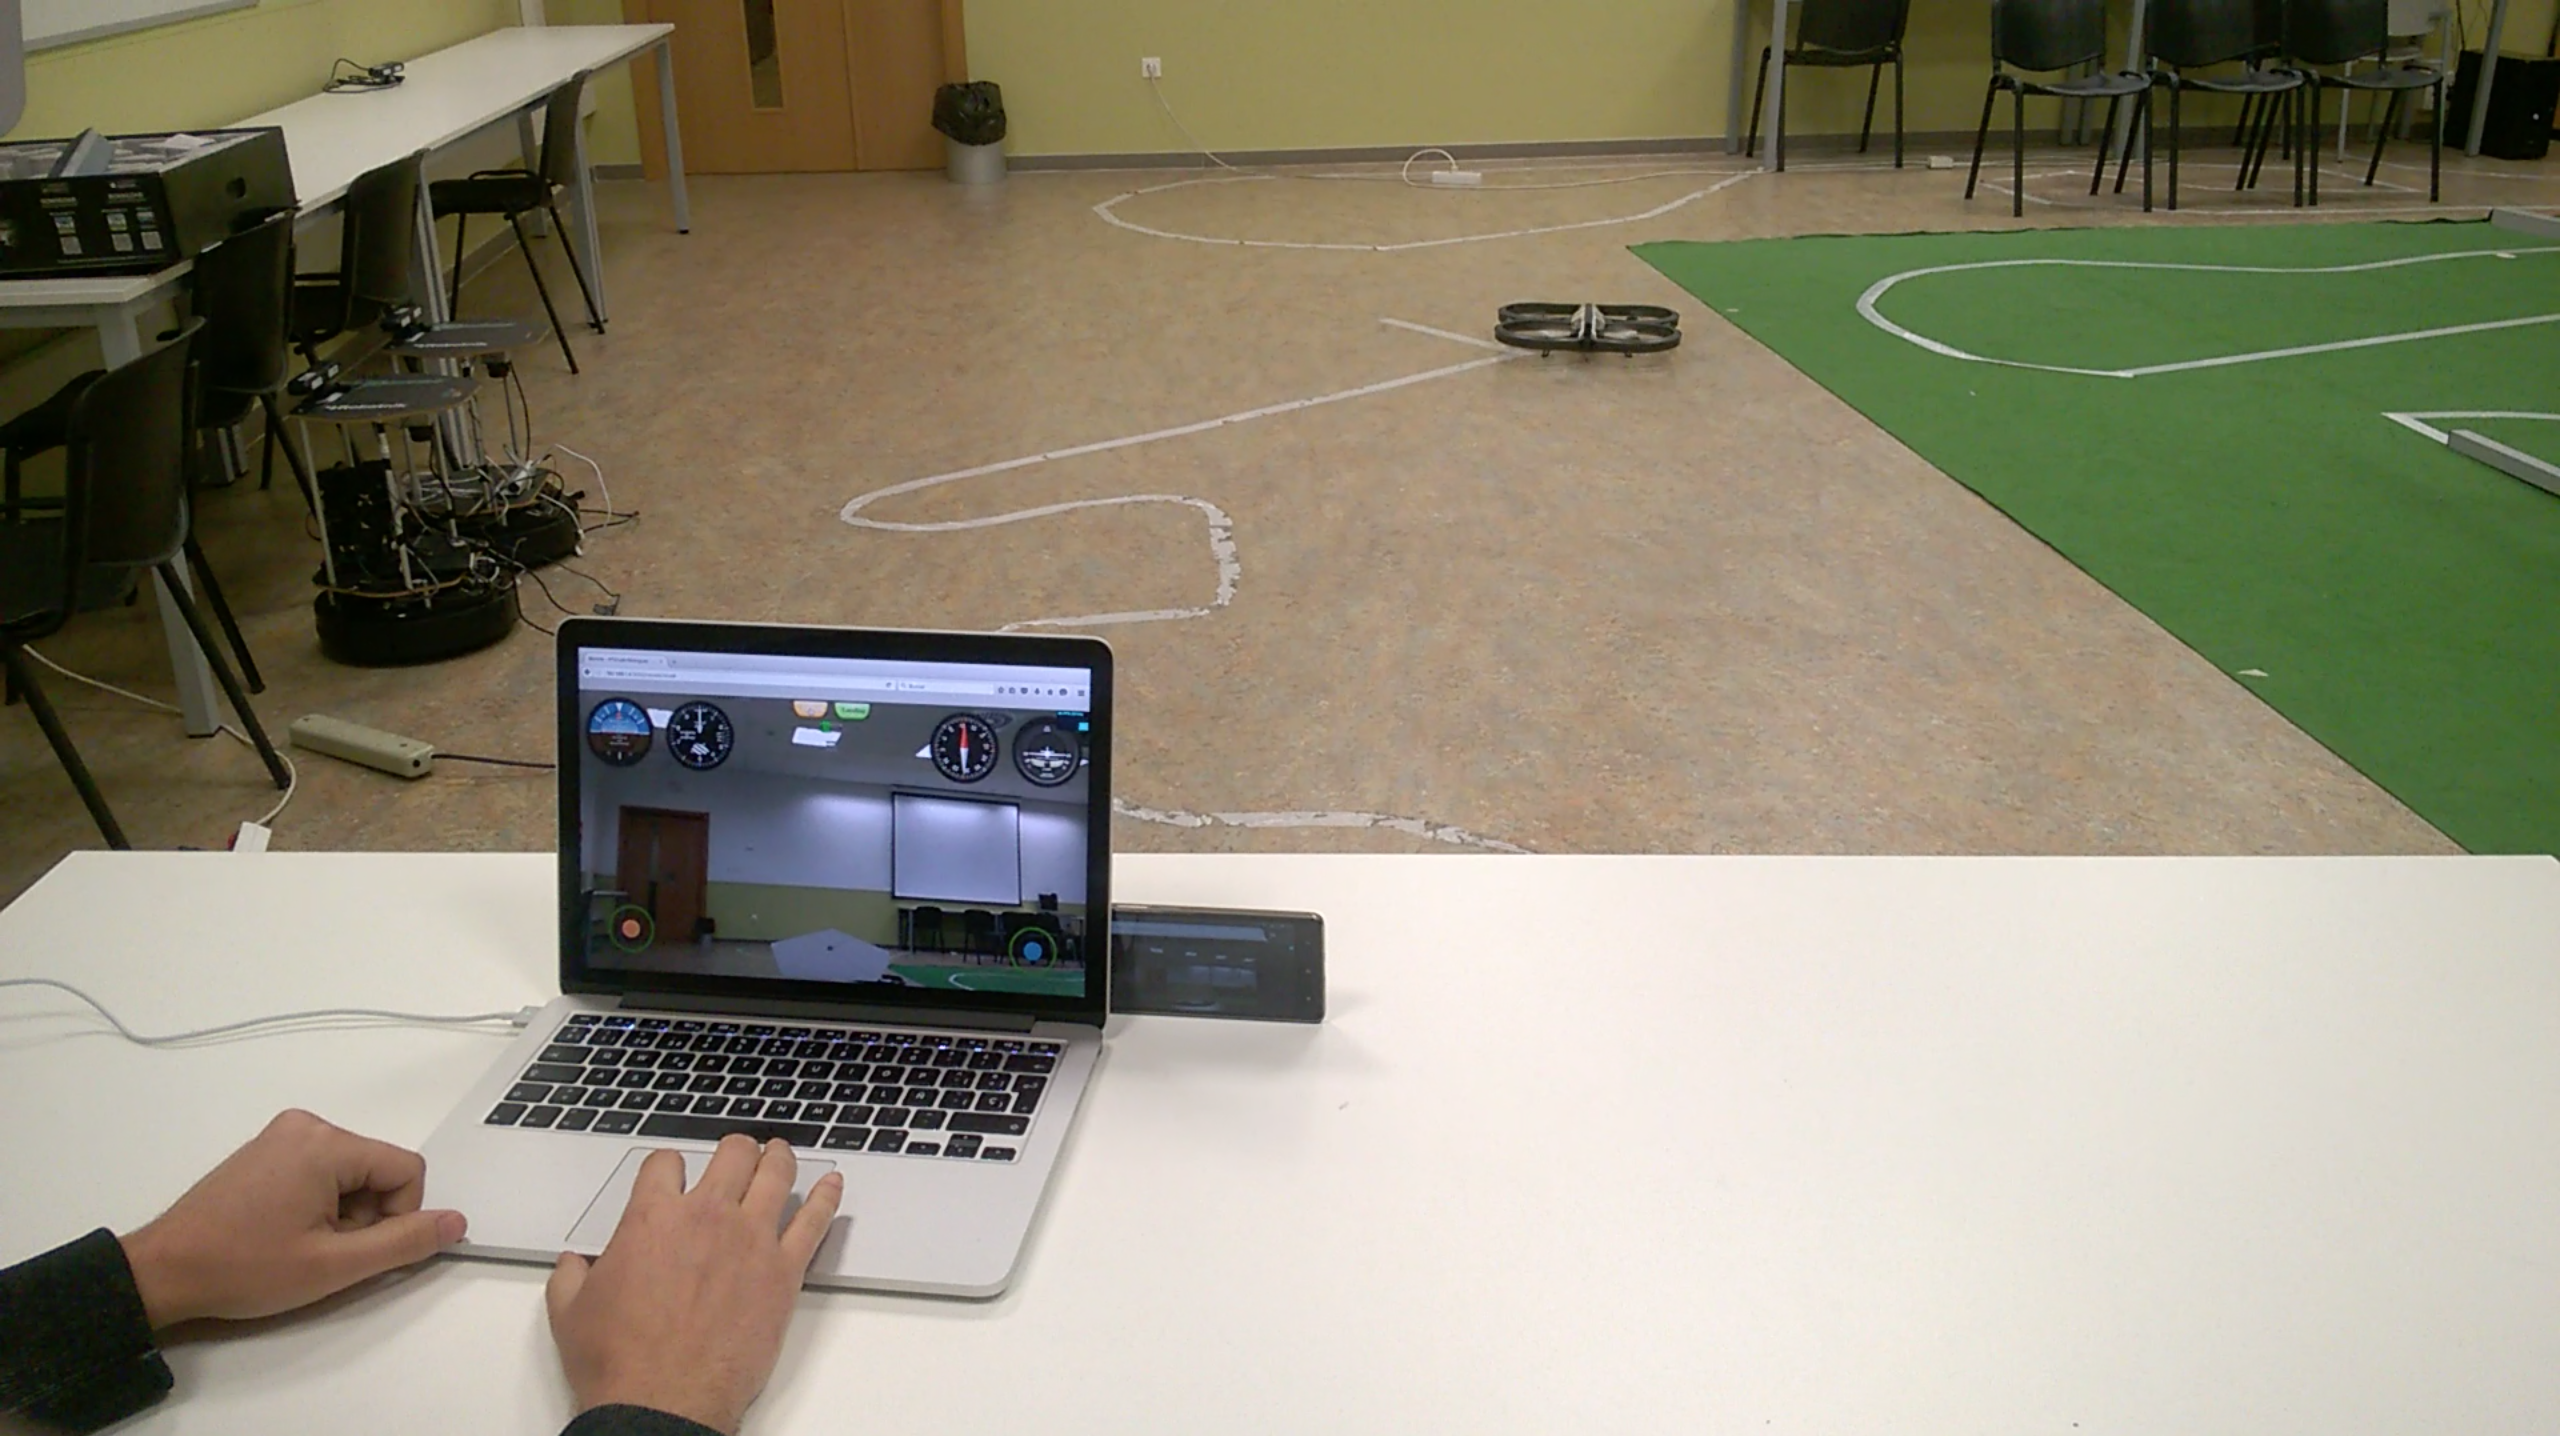
\includegraphics[width=48mm]{sec_exp4_1}
  \end{subfigure}
  \hspace{1pt}
  \begin{subfigure}[]{48mm}
    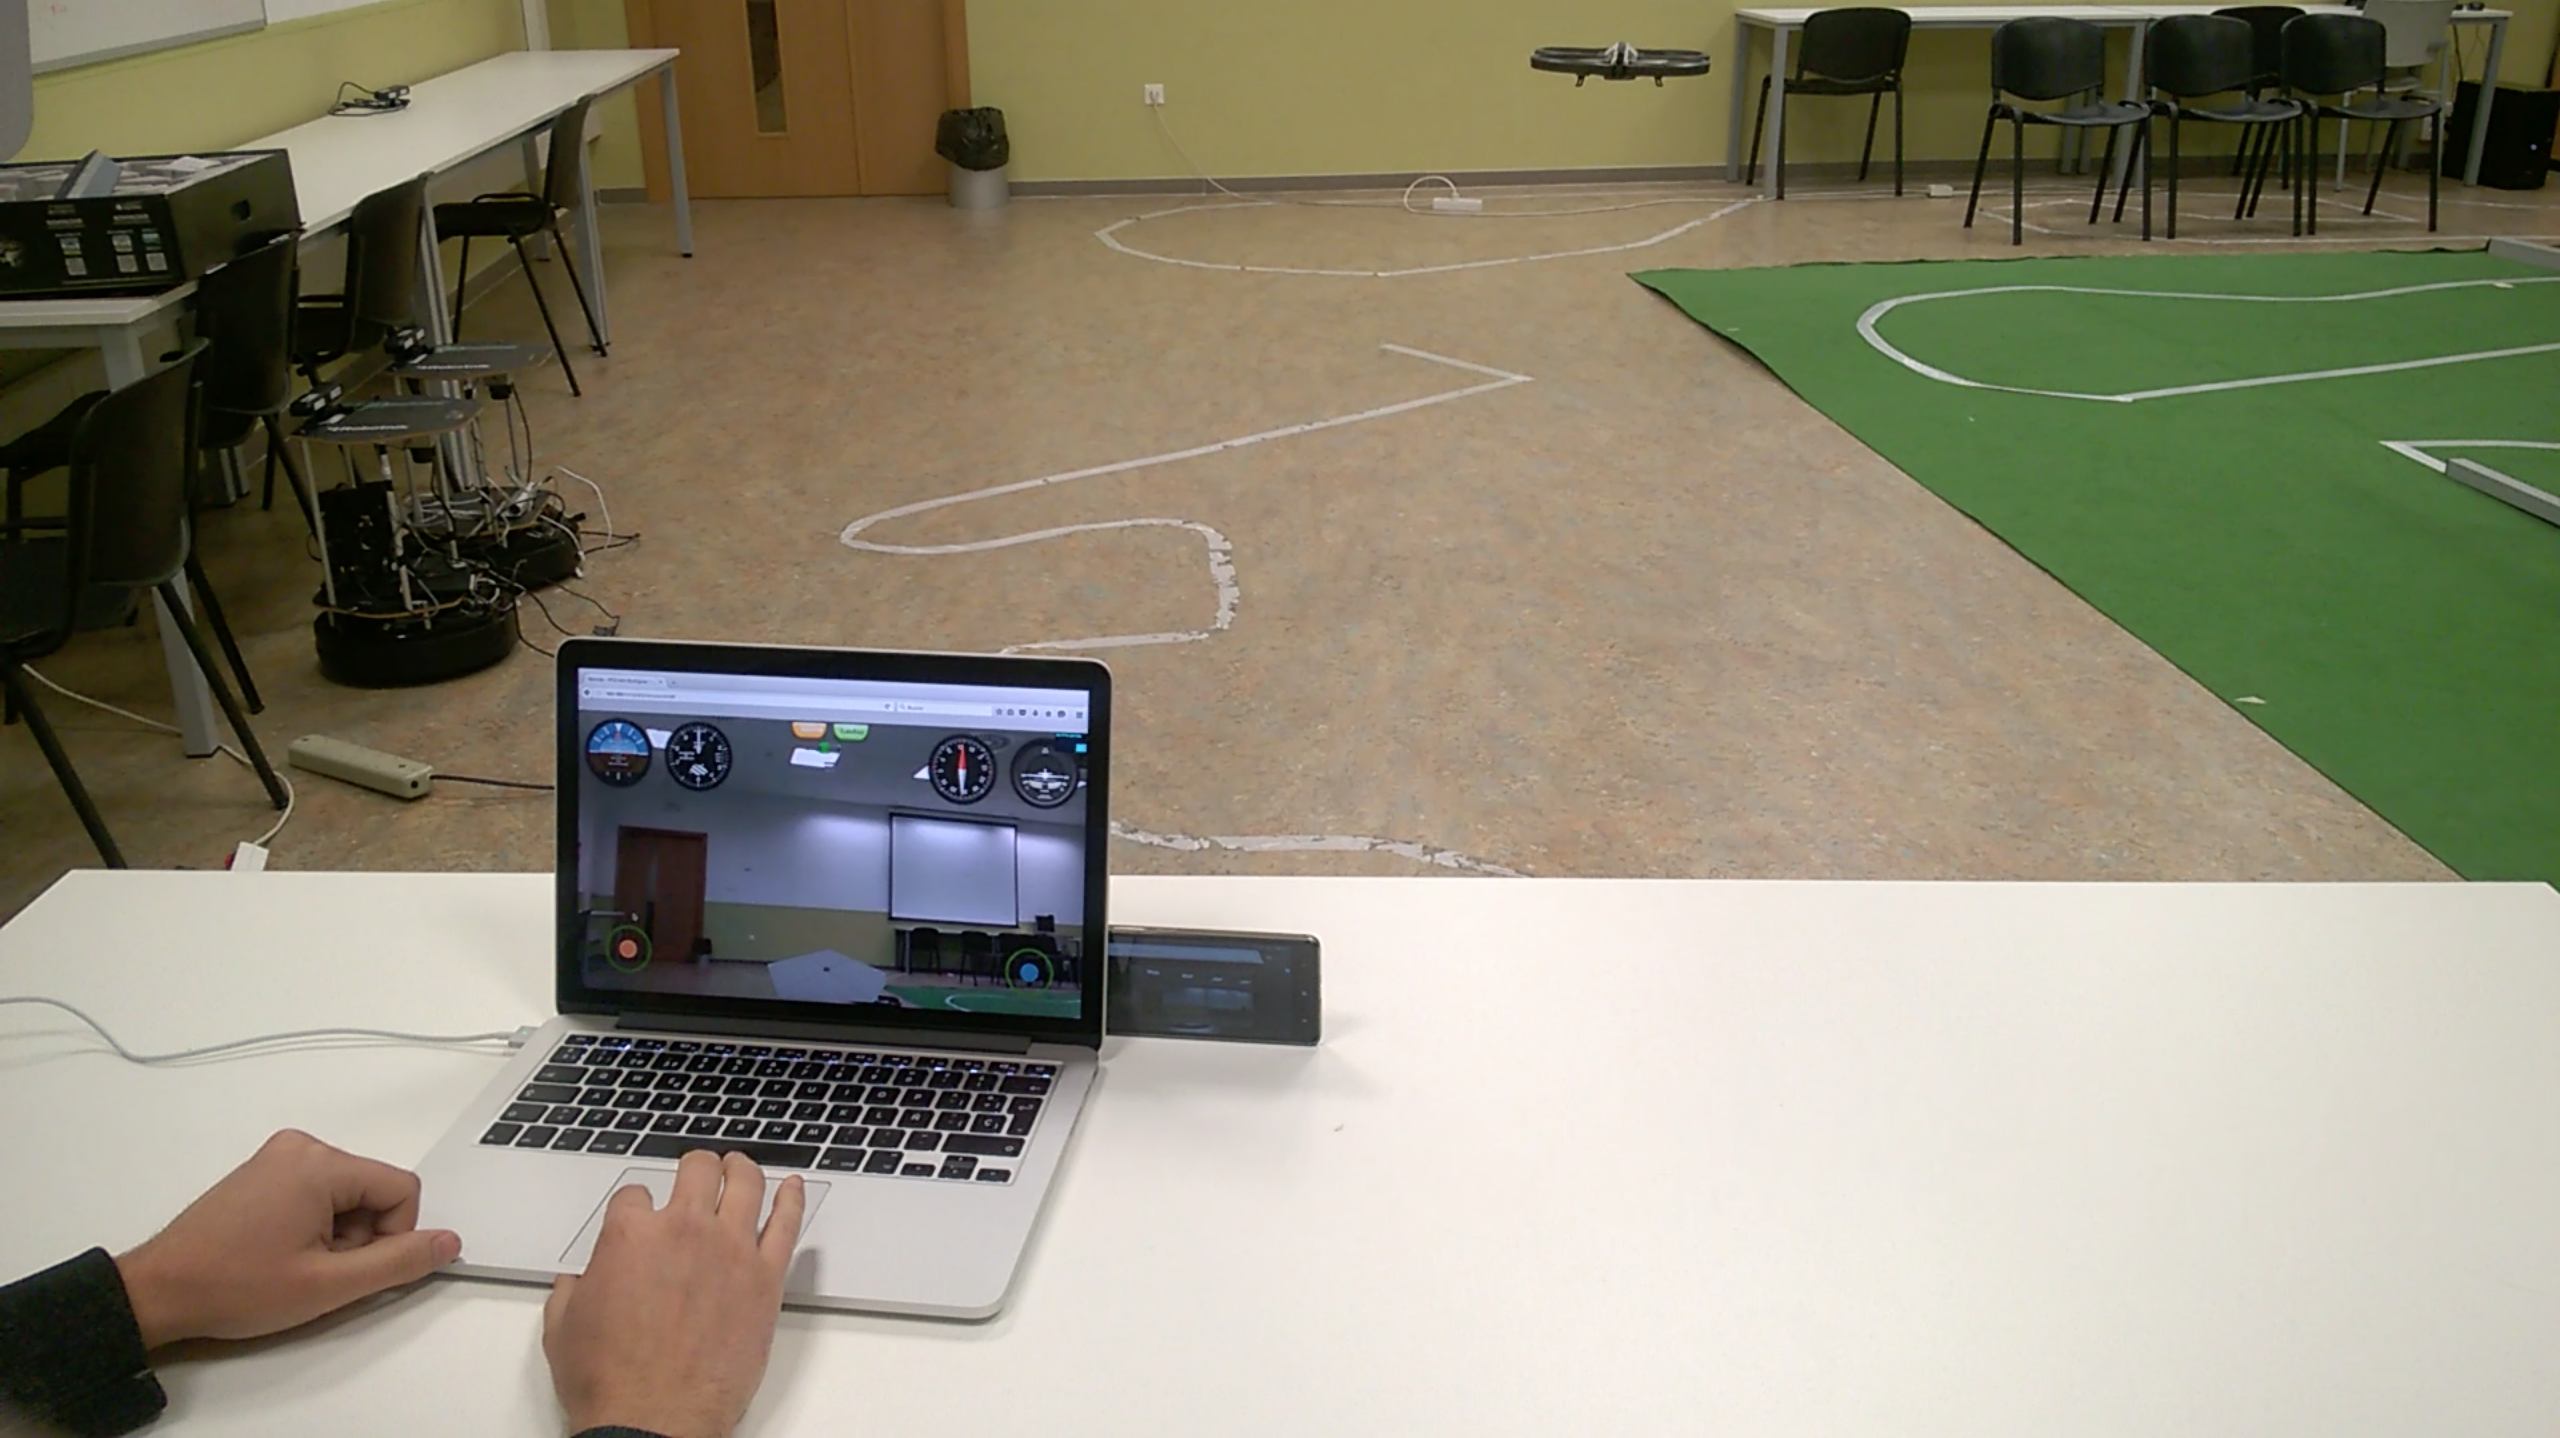
\includegraphics[width=48mm]{sec_exp4_2}
  \end{subfigure}
    \hspace{1pt}
    \begin{subfigure}[]{48mm}
    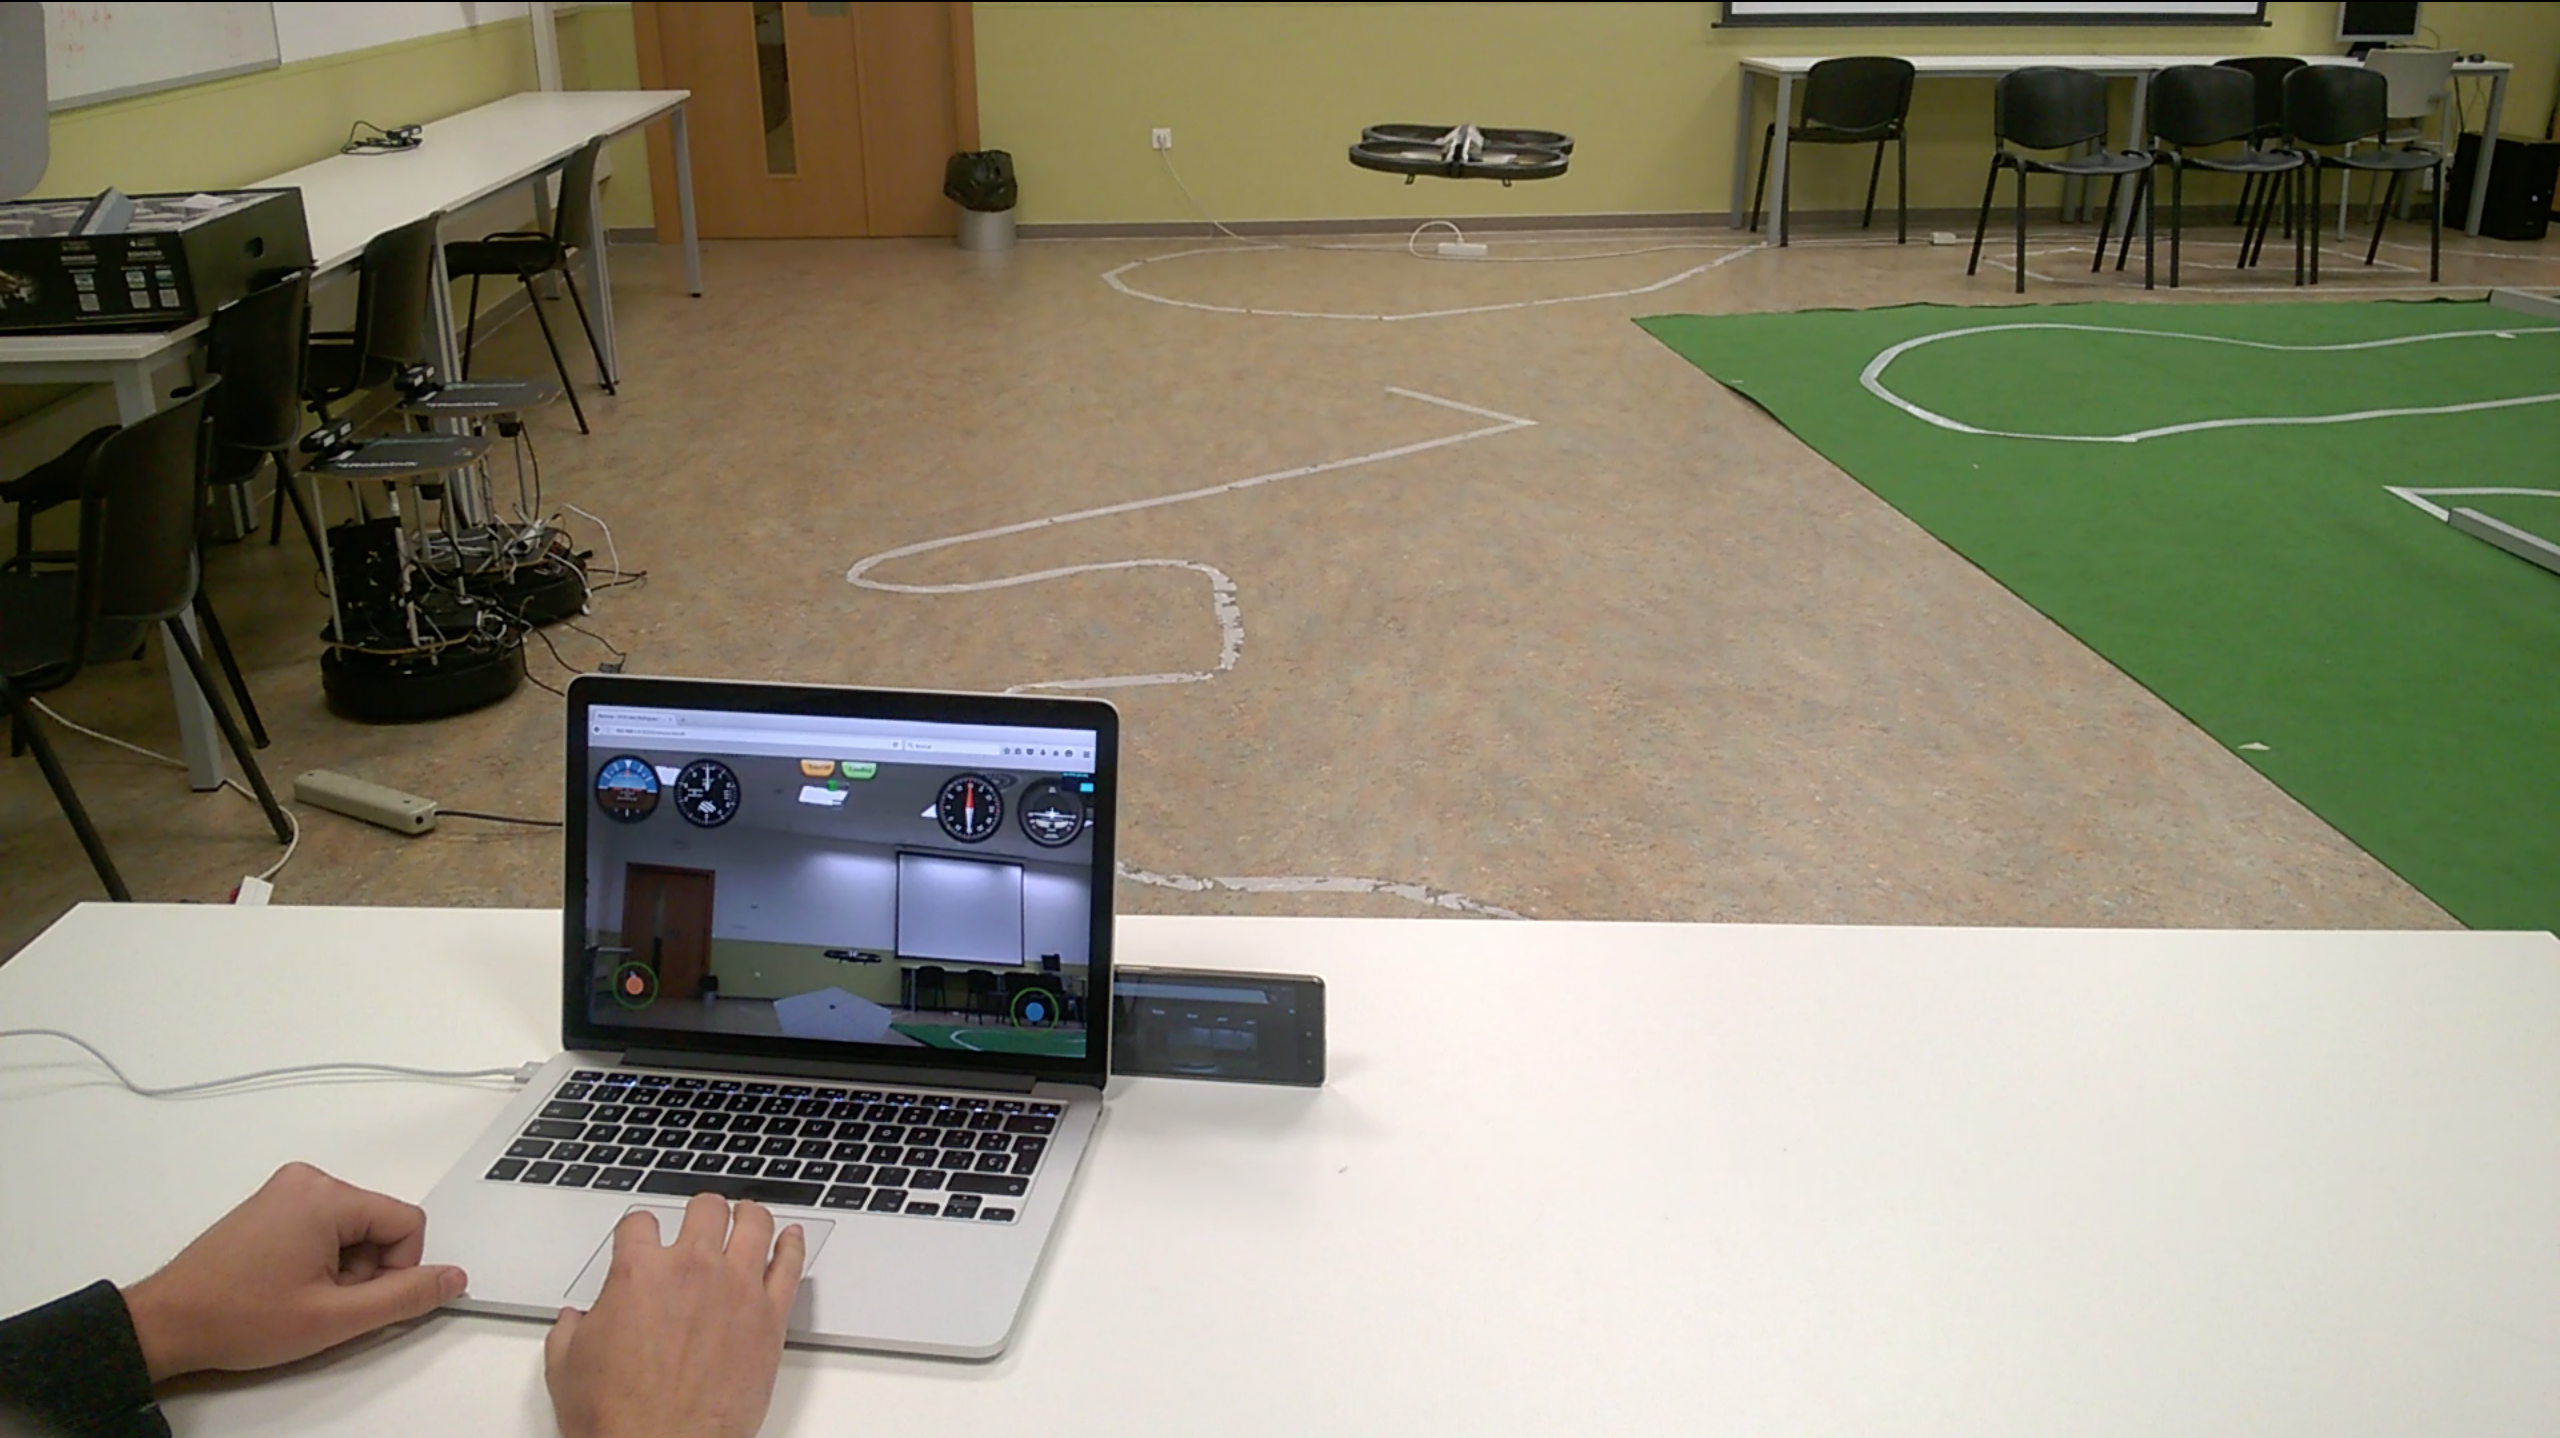
\includegraphics[width=48mm]{sec_exp4_3}
  \end{subfigure}
    \caption{Secuencia de movimiento del experimento con dispositivo móvil como par local.}
  \label{fig:secexp4}
\end{figure}

Se ha desestimado la realización del experimento en el que situamos el móvil a bordo del drone debido a la dificultad de colocarlo en posición vertical para que la cámara apunte desde la parte delantera del drone. La única posición dónde podría colocarse es en un extremo del cuadricóptero lo que causaría una descompensación de cargas dando lugar a que el drone no pudiese estabilizar el vuelo.\\


\chapter{Conclusiones}

En capítulos anteriores hemos descrito el contexto y el problema que abordamos en este proyecto, la solución propuesta junto con una serie de pruebas y experimentos que validan y software desarrollado. En este capítulo se exponen las conclusiones obtenidas y las posibles líneas por las que se puede continuar el trabajo.\\

\section{Conclusiones}

Bajo una mirada retrospectiva se puede observar que se han cumplido satisfactoriamente los objetivos generales que nos habíamos marcado. Hemos creado una aplicación web entre navegadores sin servidores intermedios que nos permite controlar, manejar y monitorizar un cuadricóptero desde un navegador, por ejemplo un teléfono móvil. Dentro de este objetivo nos marcamos tres subjetivos, los cuáles también hemos cumplido:\\

\begin{itemize}
\item Hemos creado una conexion local directamente con los sensores y actuadores del drone mediante un navegador web sin necesidad de servidores intermedios utilizando \emph{getUserMedia} de WebRTC para la cámara y ICE con \emph{WebSockets} para comunicar el navegador con el servidor JdeRobot para el drone (\texttt{ardrone\_server}).
\item Se ha desarrollado una conexión entre navegadores que transfieren en tiempo real y sin servidores intermedios la cámara y los datos necesarios para monitorar los sensores del drone y teleoperarlo. Para ello se ha utilizado \emph{RTCPeerConnection} para el vídeo y \emph{RTCDataChannel} para transmitir los datos de los sensores del drone desde el par local hacia el par remoto y en sentido opuesto las órdenes dadas por el usuario final.
\item Se ha creado una interfaz web amigable que nos permite monitorar la cámara y los sensores del drone, así como teleoperarlo de una manera muy intuitiva y sencilla de usar. Esta interfaz consta de un vídeo de fondo a pantalla completa, unos relojes de navegación dónde se representan los datos recibidos de los sensores del drone, unos \emph{joystick} virtuales para controlar el drone y un visor 3D.
\end{itemize} 

A parte de estos subobjetivos se le han añadido unos extras, como poder teleoperarlo con un mando o que tanto la conexión local como remota, así como la interfaz sean multiplataforma y multidispositivo, lo que nos permite controlarlo desde un teléfono móvil o tableta, por ejemplo.\\

Todo lo desarrollado se ha validado experimentalmente tal y como se muestra en el capítulo 5.\\

Se puede encontrar tanto esta memoria, como el repositorio del código, vídeos, explicaciones, ejemplos y resultados obtenidos en la mediawiki oficial del proyecto\footnote{\url{http://jderobot.org/Irodmar-tfg}}\cite{Mediawiki}.\\

\section{Trabajos futuros}

A todo proyecto hay que ponerle unos límites y este no es una excepción. Sirve como base y punto de partida para otros proyectos o trabajos con los que ampliar esta aplicación. Dentro de las lineas de desarrollo que se podrían seguir exponemos algunas de ellas:\\

Uno de las líneas más útiles de desarrollo podría ser incorporar diversas cámaras al drone y tener la posibilidad en el par remoto de cambiar entre ellas según nuestras necesidades.\\

Un paso más podría ser dotar al drone de autonomía, pudiendo indicarle desde el ordenador remoto unas coordenadas para que el drone se desplazase de una a otra como si de un circuito se tratase. Esto pasa por desarrollar un autopiloto dentro del cuadricóptero que le dote de capacidades de navegación autónoma.\\

Asimismo este proyecto podría integrarse en el repositorio oficial de JdeRobot\cite{jderobot_repo} desde dónde se podrá seguir trabajando en estas lineas de desarrollo o cualquier otra según las necesidades que vayan surgiendo.\\


\begin{thebibliography}{}

\bibitem{Mediawiki} Mediawiki oficial del proyecto (WebRTC en un drone) \url{http://jderobot.org/Irodmar-tfg}
\bibitem{Repositorio} Repositorio oficial del proyecto (WebRTC en un Drone) \url{https://github.com/RoboticsURJC-students/2015-tfg-irodmar} 
\bibitem{jderobot} Proyecto JdeRobot \url{http://jderobot.org/} 
\bibitem{jderobot_repo} Repositorio de JdeRobot \url{https://github.com/RoboticsURJC/JdeRobot} 
\bibitem{ArDroneServer} Mediawiki de Alberto Martín (ArDroneServer) \url{http://jderobot.org/Amartinflorido-tfg}
\bibitem{surveillance4.0} Mediawiki Daniel Castellano (Surveillance 4.0) \url{http://jderobot.org/D.castellanob-pfc} 
\bibitem{surveillance5.1} Mediawiki Edgar Barrero (Surveillance 5.1) \url{http://jderobot.org/Aerobeat-colab}
\bibitem{teleoperadoresyvisoresweb} Mediawiki Aitor Martínez \url{http://jderobot.org/Aitormf-tfg}
\bibitem{Pagina WebRTC} Página oficial de WebRTC \url{https://webrtc.org}
\bibitem{WebRTC} W3C: Borrador de la norma WebRTC \url{http://www.w3.org/TR/webrtc/}
\bibitem{WebRTC_book} Real-Time Communication with WebRTC \url{http://shop.oreilly.com/product/0636920030911.do}
\bibitem{orilley} Capítulo 18 (WebRTC) del libro \emph{High Performance Browser Networking} \url{http://chimera.labs.oreilly.com/books/1230000000545/ch18.html}
\bibitem {WebRTC experiment} WebRTC-experiment \url{https://www.webrtc-experiment.com}
\bibitem{JSEP} JSEP  \url{https://rtcweb-wg.github.io/jsep/}
\bibitem{JSEP2} Wikipedia: JSEP  \url{https://es.wikipedia.org/wiki/JSON}
\bibitem{Senalizacion1} Señalización en \emph{Mozilla Foundation} \url{https://developer.mozilla.org/es/docs/Web/API/WebRTC_API/Connectivity}
\bibitem{Senalizacion2} HTML5Rocks.com: Señalización \url{http://www.html5rocks.com/en/tutorials/webrtc/infrastructure/}
\bibitem{Senalizacion3} WebRTC-Experiment: Señalización \url{https://www.webrtc-experiment.com/docs/WebRTC-Signaling-Concepts.html}
\bibitem{WebRTC} Seguridad en WebRTC \url{https://rtcweb-wg.github.io/security-arch/}
\bibitem{SIP} Session Initiation Protocol \url{https://es.wikipedia.org/wiki/Session_Initiation_Protocol}
\bibitem{ORTC} ORTC \url{http://ortc.org/wp-content/uploads/2015/10/ortc.html}
\bibitem{jqueryflightindicator} Relojes de navegación \url{http://sebmatton.github.io/flightindicators/}
\bibitem{bateria} Repositorio batería HTML5 y CSS3 \url{http://codepen.io/jkantner/pen/QybzKL}
\bibitem{gazebo} Página oficial Gazebo \url{http://gazebosim.org/}
\bibitem{ice} Página oficial ICE  \url{http://www.zeroc.com/}
\bibitem{ice_manual}Ice 3.5.1 Documentation  \url{https://doc.zeroc.com/display/Ice35/Home}
\bibitem{slicecomp} Uso de los compiladores de Slice \url{https://doc.zeroc.com/display/Ice36/Using+the+Slice+Compilers}
\bibitem{icejs} Página de Ice for Javascript  \url{https://zeroc.com/labs/icejs/index.html}
\bibitem{icews} Websockets en ICE \url{https://zeroc.com/labs/icejs/websocket.html}
\bibitem{threejs} Página de Three.js \url{http://threejs.org/}
\bibitem{threejs_doc} Documentación de Three.js \url{http://mrdoob.github.io/three.js/docs/}
\bibitem{threejs_curso} Curso de Three.js \url{http://stemkoski.github.io/Three.js/}
\bibitem{jquery} Página de JQuery \url{https://jquery.com/}

\end{thebibliography} 



\end{document}